%beamer

% Comment/uncomment this line to toggle handout mode
%\newcommand{\handout}{}

%% Beamer-Klasse im korrekten Modus
\ifdefined \handout
\documentclass[handout]{beamer} % Handout mode
\else
\documentclass{beamer}
\fi

%% UTF-8-Encoding
\usepackage[utf8]{inputenc}

% % \bigtimes abgeschrieben von http://tex.stackexchange.com/questions/14386/importing-a-single-symbol-from-a-different-font
% \DeclareFontFamily{U}{mathx}{\hyphenchar\font45}
% \DeclareFontShape{U}{mathx}{m}{n}{
%       <5> <6> <7> <8> <9> <10> gen * mathx
%       <10.95> mathx10 <12> <14.4> <17.28> <20.74> <24.88> mathx12
%       }{}
% \DeclareSymbolFont{mathx}{U}{mathx}{m}{n}
% \DeclareMathSymbol{\bigtimes}{\mathop}{mathx}{161}

\RequirePackage{xcolor}

\def\9{\square}
%\def\9{\blank}

% f"ur Aussagenlogik
\colorlet{alcolor}{blue}
\RequirePackage{tikz}
\usetikzlibrary{arrows.meta}
\newcommand{\alimpl}{\mathrel{\tikz[x={(0.1ex,0ex)},y={(0ex,0.1ex)},>={Classical TikZ Rightarrow[]}]{\draw[alcolor,->,line width=0.7pt,line cap=round] (0,0) -- (15,0);\path (0,-6);}}}
\newcommand{\aleqv}{\mathrel{\tikz[x={(0.1ex,0ex)},y={(0ex,0.1ex)},>={Classical TikZ Rightarrow[]}]{\draw[alcolor,<->,line width=0.7pt,line cap=round] (0,0) -- (18,0);\path (0,-6);}}}
\newcommand{\aland}{\mathbin{\raisebox{-0.6pt}{\rotatebox{90}{\texttt{\color{alcolor}\char62}}}}}
\newcommand{\alor}{\mathbin{\raisebox{-0.8pt}{\rotatebox{90}{\texttt{\color{alcolor}\char60}}}}}
%\newcommand{\ali}[1]{_{\mathtt{\color{alcolor}#1}}}
\newcommand{\alv}[1]{\mathtt{\color{alcolor}#1}}
\newcommand{\alnot}{\mathop{\tikz[x={(0.1ex,0ex)},y={(0ex,0.1ex)}]{\draw[alcolor,line width=0.7pt,line cap=round,line join=round] (0,0) -- (10,0) -- (10,-4);\path (0,-8) ;}}}
\newcommand{\alP}{\alv{P}} %ali{#1}}
%\newcommand{\alka}{\negthinspace\hbox{\texttt{\color{alcolor}(}}}
\newcommand{\alka}{\negthinspace\text{\texttt{\color{alcolor}(}}}
%\newcommand{\alkz}{\texttt{\color{alcolor})}}\negthinspace}
\newcommand{\alkz}{\text{\texttt{\color{alcolor})}}\negthinspace}
\newcommand{\AAL}{A_{AL}}
\newcommand{\LAL}{\hbox{\textit{For}}_{AL}}
\newcommand{\AxAL}{\hbox{\textit{Ax}}_{AL}}
\newcommand{\AxEq}{\hbox{\textit{Ax}}_{Eq}}
\newcommand{\AxPL}{\hbox{\textit{Ax}}_{PL}}
\newcommand{\AALV}{\hbox{\textit{Var}}_{AL}}
\newcommand{\MP}{\hbox{\textit{MP}}}
\newcommand{\GEN}{\hbox{\textit{GEN}}}
\newcommand{\W}{\ensuremath{\hbox{\textbf{w}}}\xspace}
\newcommand{\F}{\ensuremath{\hbox{\textbf{f}}}\xspace}
\newcommand{\WF}{\ensuremath{\{\W,\F\}}\xspace}
\newcommand{\val}{\hbox{\textit{val}}}
\newcommand{\valDIb}{\val_{D,I,\beta}}

\newcommand*{\from}{\colon}

% die nachfolgenden Sachen angepasst an cmtt
\newlength{\ttquantwd}
\setlength{\ttquantwd}{1ex}
\newlength{\ttquantht}
\setlength{\ttquantht}{6.75pt}
\def\plall{%
  \tikz[line width=0.67pt,line cap=round,line join=round,baseline=(B),alcolor] {
    \draw (-0.5\ttquantwd,\ttquantht) -- node[coordinate,pos=0.4] (lll){} (-0.25pt,-0.0pt) -- (0.25pt,-0.0pt) -- node[coordinate,pos=0.6] (rrr){} (0.5\ttquantwd,\ttquantht);
    \draw (lll) -- (rrr);
    \coordinate (B) at (0,-0.35pt);
  }%
}
\def\plexist{%
  \tikz[line width=0.67pt,line cap=round,line join=round,baseline=(B),alcolor] {
    \draw (-0.9\ttquantwd,\ttquantht) -- (0,\ttquantht) -- node[coordinate,pos=0.5] (mmm){} (0,0) --  (-0.9\ttquantwd,0);
    \draw (mmm) -- ++(-0.75\ttquantwd,0);
    \coordinate (B) at (0,-0.35pt);
  }\ensuremath{\,}%
}
\let\plexists=\plexist
\newcommand{\NT}[1]{\ensuremath{\langle\mathrm{#1} \rangle}}

\newcommand{\CPL}{\text{\itshape Const}_{PL}}
\newcommand{\FPL}{\text{\itshape Fun}_{PL}}
\newcommand{\RPL}{\text{\itshape Rel}_{PL}}
\newcommand{\VPL}{\text{\itshape Var}_{PL}}
\newcommand{\ATer}{A_{\text{\itshape Ter}}}
\newcommand{\ARel}{A_{\text{\itshape Rel}}}
\newcommand{\AFor}{A_{\text{\itshape For}}}
\newcommand{\LTer}{L_{\text{\itshape Ter}}}
\newcommand{\LRel}{L_{\text{\itshape Rel}}}
\newcommand{\LFor}{L_{\text{\itshape For}}}
\newcommand{\NTer}{N_{\text{\itshape Ter}}}
\newcommand{\NRel}{N_{\text{\itshape Rel}}}
\newcommand{\NFor}{N_{\text{\itshape For}}}
\newcommand{\PTer}{P_{\text{\itshape Ter}}}
\newcommand{\PRel}{P_{\text{\itshape Rel}}}
\newcommand{\PFor}{P_{\text{\itshape For}}}

\newcommand{\plka}{\alka}
\newcommand{\plkz}{\alkz}
%\newcommand{\plka}{\plfoo{(}}
%\newcommand{\plkz}{\plfoo{)}}
\newcommand{\plcomma}{\hbox{\texttt{\color{alcolor},}}}
\newcommand{\pleq}{{\color{alcolor}\,\dot=\,}}

% MODIFIED (DJ)
% previously: \newcommand{\plfoo}[1]{\mathtt{\color{alcolor}#1}}
\newcommand{\plfoo}[1]{\texttt{\color{alcolor}#1}}

\newcommand{\plc}{\plfoo{c}}
\newcommand{\pld}{\plfoo{d}}
\newcommand{\plf}{\plfoo{f}}
\newcommand{\plg}{\plfoo{g}}
\newcommand{\plh}{\plfoo{h}}
\newcommand{\plx}{\plfoo{x}}
\newcommand{\ply}{\plfoo{y}}
\newcommand{\plz}{\plfoo{z}}
\newcommand{\plR}{\plfoo{R}}
\newcommand{\plS}{\plfoo{S}}

\newcommand{\bv}{\mathrm{bv}}
\newcommand{\fv}{\mathrm{fv}}

%\newcommand{\AxAL}{\hbox{\textit{Ax}}_{AL}}
%\newcommand{\AALV}{\hbox{\textit{Var}}_{AL}}

%\renewcommand{\#}[1]{\literal{#1}}
\newcommand{\A}{\mathcal{A}}
\newcommand{\Adr}{\text{Adr}}
\newcommand{\ar}{\mathrm{ar}}
\newcommand{\ascii}[1]{\literal{\char#1}}
%\newcommand{\assert}[1]{\text{/\!\!/\ } #1}
\newcommand{\assert}[1]{\colorbox{black!7!white}{\ensuremath{\{\;#1\;\}}}}
\newcommand{\Assert}[1]{$\langle$\textit{#1}$\rangle$}
\newcommand{\B}{\mathcal{B}}
\newcommand{\bfmod}{\mathbin{\kw{ mod }}}
\newcommand{\bb}{{\text{bb}}}
\def\bottom{\hbox{\small$\pmb{\bot}$}}
\newcommand{\card}[1]{|#1|}
%\newcommand{\cod}{\mathop{\text{cod}}}  % ist in thwmathabbrevs
\newcommand{\Conf}{\mathcal{C}}
\newcommand{\define}[1]{\emph{#1}}
%\renewcommand{\dh}{d.\,h.\@\xspace}
%\newcommand{\Dh}{D.\,h.\@\xspace}
%\newcommand{\engl}[1]{engl.\xspace\emph{#1}}
\newcommand{\eps}{\varepsilon}
%\newcommand{\evtl}{evtl.\@\xspace}
\newcommand{\fbin}{\text{bin}}
\newcommand{\finv}{\text{inv}}
\newcommand{\fnum}{\text{num}}
\newcommand{\fNum}{{\text{Num}}}
\newcommand{\frepr}{\text{repr}}
\newcommand{\fRepr}{\text{Repr}}
\newcommand{\fZkpl}{\text{Zkpl}}
\newcommand{\fLen}{\text{Len}}
\newcommand{\fsem}{\text{sem}}
\providecommand{\fspace}{\mathord{\text{space}}}
\providecommand{\fSpace}{\mathord{\text{Space}}}
\providecommand{\ftime}{\mathord{\text{time}}}
\providecommand{\fTime}{\mathord{\text{Time}}}
\newcommand{\fTrans}{\text{Trans}}
\newcommand{\fVal}{\text{Val}}

% MODIFIED (DJ)
\newcommand{\Val}{\text{Val}}

%\def\G{\mathbb{Z}}
\newcommand{\HT}[1]{\normalfont\textsc{HT-#1}}
\newcommand{\htr}[3]{\{#1\}\;#2\; \{#3\}}
\newcommand{\Id}{\text{I}}
%\newcommand{\ie}{i.\,e.\@\xspace}
\newcommand{\instr}[2]{\texttt{#1}\ \textit{#2}}
\newcommand{\Instr}[2]{\texttt{#1}\ \textrm{#2}}
\newcommand{\instrr}[3]{\texttt{#1}\ \textit{#2}\texttt{(#3)}}
\newcommand{\Instrr}[3]{\texttt{#1}\ \textrm{#2}\texttt{(#3)}}

% MODIFIED (DJ)
% previously:  \newcommand{\io}{\!\mid\!}
\newcommand{\io}{\ensuremath{\!\mid\!}}

\usepackage{KITcolors}
\newcommand{\literal}[1]{\hbox{\textcolor{blue!95!white}{\textup{\texttt{\scalebox{1.11}{#1}}}}}}
%\newcommand{\literal}[1]{\hbox{\textcolor{KITblue!80!black}{\textup{\texttt{#1}}}}}
\def\kasten#1{\leavevmode\literal{\setlength{\fboxsep}{1pt}\fbox{\vrule  width 0pt height 1.5ex depth 0.5ex #1}}}
\newcommand{\kw}[1]{\ensuremath{\mathbf{#1}}}
\newcommand{\lang}[1]{\ensuremath{\langle#1\rangle}}
%\newcommand{\maw}{m.\,a.\,w.\@\xspace}
%\newcommand{\MaW}{M.\,a.\,w.\@\xspace}
\newcommand{\mdefine}[2][FOOBAR]{\define{#2}\def\foobar{FOOBAR}\def\optarg{#1}\ifx\foobar\optarg\def\optarg{#2}\fi\graffito{\optarg}}
\newcommand{\meins}{\rotatebox[origin=c]{180}{1}}
\newcommand{\Mem}{\text{Mem}}
\newcommand{\memread}{\text{memread}}
\newcommand{\memwrite}{\text{memwrite}}
\providecommand{\meta}[1]{\ensuremath{\langle}\textit{#1}\ensuremath{\rangle}}
%\newcommand{\N}{\mathbb{N}}
\newcommand{\NP}{\mathbf{NP}}
\newcommand{\Nadd}{N_{\text{add}}}
\newcommand{\Nmult}{N_{\text{mult}}}
% MODIFIED (DJ): added \!, mathcal{O}
\newcommand{\Oh}[1]{\mathcal{O}\!\left(#1\right)}
\newcommand{\Om}[1]{\Omega\!\left(#1\right)}
\newcommand{\personname}[1]{\textsc{#1}}
\newcommand{\regname}[1]{\texttt{#1}}
\newcommand{\mima}{\textsc{Mima}\xspace}
\newcommand{\mimax}{\textsc{Mima-X}\xspace}

\def\Pclass{\text{\bfseries P}}
\def\PSPACE{\text{\bfseries PSPACE}}

\newcommand{\SPush}{\text{push}}
\newcommand{\SPop}{\text{pop}}
\newcommand{\SPeek}{\text{peek}}
\newcommand{\STop}{\text{top}}
\newcommand{\STos}{\text{\itshape tos}}
\newcommand{\SBos}{\text{\itshape bos}}

%\newcommand{\R}{\mathbb{R}}
\newcommand{\Rnullplus}{\R_0^{+}}
\newcommand{\Rplus}{\R_{+}}
\newcommand{\resp}{resp.\@\xspace}
\newcommand{\Sem}{\text{Sem}}
\newcommand{\sgn}{\mathop{\text{sgn}}}
\newcommand{\sqbox}{\mathop{\raisebox{-6.2pt}{\hbox{\hbox to 0pt{$^{^{\sqcap}}$\hss}$^{^{\sqcup}}$}}}}
\newcommand{\sqleq}{\sqsubseteq}
\newcommand{\sqgeq}{\sqsupseteq}
% MODIFIED (DJ): added \!
\newcommand{\Th}[1]{\Theta\!\left(#1\right)}
%\newcommand{\usw}{usw.\@\xspace}
\newcommand{\V}[1]{\hbox{\textit{#1}}}
\newcommand{\x}{\times}
\newcommand{\ZK}{\mathbb{K}}
%\newcommand{\Z}{\mathbb{Z}}
\newcommand{\zB}{z.\,B.\@\xspace}
\newcommand{\ZB}{Z.\,B.\@\xspace}
% \newcommand{\bb}{{\text{bb}}}
% \def\##1{\hbox{\textcolor{darkblue}{\texttt{#1}}}}
% \def\A{\mathcal{A}}
% \newcommand{\0}{\#0}
% \newcommand{\1}{\#1}
% \newcommand{\Obj}{\text{Obj}}
% \newcommand{\start}{\mathop{\text{start}}}
% \newcommand{\compactlist}{\addtolength{\itemsep}{-\parskip}}
% \newcommand{\fval}{\text{val}}
% \newcommand{\lang}[1]{\ensuremath{\langle#1\rangle}}
% \newcommand{\io}{\!\mid\!}
% \def\sqbox{\mathop{\raisebox{-6.2pt}{\hbox{\hbox to 0pt{$^{^{\sqcap}}$\hss}$^{^{\sqcup}}$}}}}
% \def\sqleq{\sqsubseteq}
% \def\sqgeq{\sqsupseteq}
\def\Td{T_{\overline{d}}}
% \newcommand{\csym}[1]{\ensuremath{\#{c}_{\#{\hbox{\scriptsize #1}}}}}
% \newcommand{\F}{\ensuremath{\mathcal{F}}}
% \newcommand{\fsym}[2]{\ensuremath{\#{f}^{\#{\hbox{\scriptsize #1}}}_{\#{\hbox{\scriptsize #2}}}}}
% \newcommand{\rsym}[2]{\ensuremath{\#{R}^{\#{\hbox{\scriptsize #1}}}_{\#{\hbox{\scriptsize #2}}}}}
% \newcommand{\xsym}[1]{\ensuremath{\#{x}_{\#{\hbox{\scriptsize #1}}}}}
% \newcommand{\I}{\mathcal{I}}
% ********************************************************************

\usepackage[blue]{../framework/thwregex}
\usepackage{environ}
\usepackage{bm}
\usepackage{calc}
\usepackage{varwidth}
\usepackage{wasysym}
\usepackage{mathtools}

%%%%%%%%%%%%%%%%%%%%%%%%%%%%%%%%%%%% Copied from Style_Tut.tex


% Das ist der KIT-Stil
%\usepackage{../TutTexbib/beamerthemekit}
\usepackage[deutsch,titlepage0]{../framework/KIT/beamerthemeKITmod}
\TitleImage[width=\titleimagewd]{../figures/titlepage.jpg}
%\usetheme[deutsch,titlepage0]{KIT}

% Include PDFs
\usepackage{pdfpages}

% Libertine font (Original GBI font)
\usepackage{libertine}
%\renewcommand*\familydefault{\sfdefault}  %% Only if the base font of the document is to be sans serif

% Nicer math symbols
\usepackage{eulervm}
%\usepackage{mathpazo}
\renewcommand\ttdefault{cmtt} % Computer Modern typewriter font, see lecture slides.

\usepackage{csquotes}

%%%%%%

%% Schönere Schriften
\usepackage[TS1,T1]{fontenc}

%% Bibliothek für Graphiken
\usepackage{graphicx}

%% der wird sowieso in jeder Datei gesetzt
%%\graphicspath{{../figures/}}

%% Anzeigetiefe für Inhaltsverzeichnis: 1 Stufe
\setcounter{tocdepth}{1}

%% Hyperlinks
\usepackage{hyperref}
% I don't know why, but this works and only includes sections and NOT subsections in the pdf-bookmarks.
\hypersetup{bookmarksdepth=subsection} 

%\usepackage{lmodern}
\usepackage{colortbl}
\usepackage[absolute,overlay]{textpos}
\usepackage{listings}
\usepackage{forloop}
%\usepackage{algorithmic} % PseudoCode package 

\usepackage{tikz}
\usetikzlibrary{matrix}
\usetikzlibrary{arrows.meta}
\usetikzlibrary{automata}
\usetikzlibrary{tikzmark}

% Needed for gbi-macros
\usepackage{xspace}

%%%%%%

%% Verbatim
\usepackage{moreverb}

%%%%%%%%%%%%%%%%%%%%%%%%%%%%%%%%%%%% Copy end

%% Tabellen
\usepackage{array}
\usepackage{multicol}

%% Bibliotheken für viele mathematische Symbole
\usepackage{amsmath, amsfonts, amssymb}

%% Deutsche Silbentrennung und Beschriftungen
\usepackage[ngerman]{babel}

\usepackage{kbordermatrix}

% kbordermatrix settings
\renewcommand{\kbldelim}{(} % Left delimiter
\renewcommand{\kbrdelim}{)} % Right delimiter


% This is a configuration file with personal tutor information.
% It is therefore excluded from the git repository, so changes in this file will not conflict in git commits.

% Copy this template, rename to config.tex and add your information below.

\newcommand{\myname}{Lukas Morawietz}
\newcommand{\mymail}{lukas.morawietz@gmail.com} % Consider using your named student mail address to keep your u**** account private.
\newcommand{\mytutnumber}{31}

% Don't forget to update ILIAS url. WARNING: Underscores '_' and Ampersands '&' have to be escaped with backslashes '\'. Blame TeX, not me.
\newcommand{\myILIASurl}{https://ilias.studium.kit.edu/ilias.php?ref\_id=855240\&cmdClass=ilrepositorygui\&cmdNode=5r\&baseClass=ilrepositorygui}

% Uncommenting this will print Socrative info with here defined roomname whenever \Socrative is called.
% (Otherwise, \Socrative will remain silent.)
% \newcommand{\mysocrativeroom}{???}

%\def\ThassesTut{}
\def\DanielsTut{}

\newcommand{\aboutMeFrame}{
	\begin{frame}{Über mich}
		\myname \\
		Informatik, 9. Fachsemester (Bachelor)
		% Lebensgeschichte...
		% Stammbaum...
		% Aufarbeitung der eigenen Todesser-Vergangenheit...
	\end{frame}
}

\def\thisyear{2019}

% Update date of exam
\def\myKlausurtermin{18.~März~2020, 14:00–16:00~Uhr}

\def\mydate#1{
		  \ifnum#1=1\relax	  23. Oktober \thisyear \
	\else \ifnum#1=2\relax	  30. Oktober \thisyear \
	\else \ifnum#1=3\relax    06. November \thisyear \
	\else \ifnum#1=4\relax    13. November \thisyear \
	\else \ifnum#1=5\relax    20. November \thisyear \
	\else \ifnum#1=6\relax    27. November \thisyear \
	\else \ifnum#1=7\relax    04. Dezember \thisyear \
	\else \ifnum#1=8\relax    11. Dezember \thisyear \
	\else \ifnum#1=9\relax    18. Dezember \thisyear \
	\else \ifnum#1=10\relax   08. Januar \nextyear \
	\else \ifnum#1=11\relax   15. Januar \nextyear \
	\else \ifnum#1=12\relax   22. Januar \nextyear \
	\else \ifnum#1=13\relax   29. Januar \nextyear \
	\else \ifnum#1=14\relax   05. Februar \nextyear \
	\else \textbf{Datum undefiniert!} 
	\fi\fi\fi\fi\fi\fi\fi\fi\fi\fi\fi\fi\fi\fi
}

\def\mylasttimestext{Was letztes Mal geschah...}

\colorlet{beamerlightred}{red!40}
\colorlet{beamerlightgreen}{green!50}
\colorlet{beamerlightyellow}{yellow!50}
\colorlet{lightred}{red!30}
\colorlet{lightgreen}{green!40}
\colorlet{lightyellow}{yellow!50}
\colorlet{fullred}{red!60}
\colorlet{fullgreen}{green}

\definecolor{myalertcolor}{rgb}{1,0.33,0.24}
\setbeamercolor{alerted text}{fg=myalertcolor}

% Flag to toggle display of KIT Logo.
% If you want to conform to the official logo guidelines, 
% you are not allowed to use the logo and should disable it
% using the following flag. Just saying.
% (But it's too beautiful, so best leave this commented. :P)
%\newcommand{\noKITLogo}{}

% Toggle handout mode by including the following line before including PraeambelTut
% and removing the % at the start (but do NOT remove the % char here, otherwise handout mode will always be on!)
% Please keep handout mode off in all commits!

% \newcommand{\handout}{}



% define custom \handout command flag if handout mode is toggled  #DirtyAsHellButWell...
\only<beamer:0>{\def\handout{}} %beamer:0 == handout mode

\newcommand{\R}{\mathbb{R}}
\newcommand{\N}{\mathbb{N}}
\newcommand{\Z}{\mathbb{Z}}
\newcommand{\Q}{\mathbb{Q}}
\newcommand{\BB}{\mathbb{B}}
\newcommand{\C}{\mathbb{C}}
\newcommand{\K}{\mathbb{K}}
\newcommand{\G}{\mathbb{G}}
\newcommand{\nullel}{\mathcal{O}}
\newcommand{\einsel}{\mathds{1}}
\newcommand{\Pot}{\mathcal{P}}
\renewcommand{\O}{\text{O}}

\def\word#1{\hbox{\textcolor{blue}{\texttt{#1}}}}
\let\literal\word
\def\mword#1{\hbox{\textcolor{blue}{$\mathtt{#1}$}}}  % math word
\def\sp{\scalebox{1}[.5]{\textvisiblespace}}
\def\wordsp{\word{\sp}}

%\newcommand{\literal}[1]{\textcolor{blue}{\texttt{#1}}}
\newcommand{\realTilde}{\textasciitilde \ }
\newcommand{\setsize}[1]{\ensuremath{\left\lvert #1 \right\rvert}}
\newcommand{\size}[1]{\setsize{#1}}  % Shame on you, TeXStudio...
\newcommand{\set}[1]{\left\{#1\right\}}
\newcommand{\tuple}[1]{\left(#1\right)}
\newcommand{\normalvar}[1]{\text{$#1$}}

% Modified by DJ
\let\oldemptyset\emptyset
\let\emptyset\varnothing % proper emptyset

\newcommand{\boder}{\ensuremath{\mathbin{\textcolor{blue}{\vee}}}\xspace}
\newcommand{\bund}{\ensuremath{\mathbin{\textcolor{blue}{\wedge}}}\xspace}
\newcommand{\bimp}{\ensuremath{\mathrel{\textcolor{blue}{\to}}}\xspace}
\newcommand{\bgdw}{\ensuremath{\mathrel{\textcolor{blue}{\leftrightarrow}}}\xspace}
\newcommand{\bnot}{\ensuremath{\textcolor{blue}{\neg}}\xspace}
\newcommand{\bone}{\ensuremath{\textcolor{blue}{1}}\text{}}
\newcommand{\bzero}{\ensuremath{\textcolor{blue}{0}}\text{}}
\newcommand{\bleftBr}{\ensuremath{\textcolor{blue}{\texttt{(}}}\text{}}
\newcommand{\brightBr}{\ensuremath{\textcolor{blue}{\texttt{)}}}\text{}}

% Fix of \b... commands:

\renewcommand{\boder}{\alor}
\renewcommand{\bund}{\aland}
\renewcommand{\bimp}{\alimpl}
\renewcommand{\bgdw}{\aleqv}
\renewcommand{\bnot}{\alnot}
\renewcommand{\bleftBr}{\alka}
\renewcommand{\brightBr}{\alkz}
\newcommand{\alA}{\word A}
\newcommand{\alB}{\word B}
\newcommand{\alC}{\word C}

\newcommand{\plB}{\plfoo{B}}
\newcommand{\plE}{\plfoo{E}}

\newcommand{\summe}[2]{\sum\limits_{#1}^{#2}}
\newcommand{\limes}[1]{\lim\limits_{#1}}

%\newcommand{\numpp}{\advance \value{weeknum} by -2 \theweeknum \advance \value{weeknum} by 2}
%\newcommand{\nump}{\advance \value{weeknum} by -1 \theweeknum \advance \value{weeknum} by 1}

\newcommand{\mycomment}[1]{}
\newcommand{\Comment}[1]{}

%% DISCLAIMER START 
% It is INSANELY IMPORTANT NOT TO DO THIS OUTSIDE BEAMER CLASS! IN ARTCILE DOCUMENTS, THIS IS VERY LIKELY TO BUG AROUND!
\makeatletter%
\@ifclassloaded{beamer}%
{
	% TODO 
	% no time...
	% redefine section to ignore multiple \section calls with the same title
}%
{
	\errmessage{ERROR: section command redefinition outside of beamer class document! Please contact the author of this code.}
}%
\makeatother%
%% DISCLAIMER END

\newcounter{abc}
\newenvironment{alist}{
  \begin{list}{(\alph{abc})}{
      \usecounter{abc}\setlength{\leftmargin}{8mm}\setlength{\labelsep}{2mm}
    }
}{\end{list}}


\newcommand{\stdarraystretch}{1.20}
\renewcommand{\arraystretch}{\stdarraystretch}  % for proper row spacing in tables

\newcommand{\morescalingdelimiters}{   % for proper \left( \right) typography
	\delimitershortfall=-1pt  
	\delimiterfactor=1
}

\newcommand{\centered}[1]{\vspace{-\baselineskip}\begin{center}#1\end{center}\vspace{-\baselineskip}}

% for \implitem and \item[bla] stuff to look right:
\setbeamercolor*{itemize item}{fg=black}
\setbeamercolor*{itemize subitem}{fg=black}
\setbeamercolor*{itemize subsubitem}{fg=black}

\setbeamercolor*{description item}{fg=black}
\setbeamercolor*{description subitem}{fg=black}
\setbeamercolor*{description subsubitem}{fg=black}

\renewcommand{\qedsymbol}{\textcolor{black}{\openbox}}

\renewcommand{\mod}{\mathop{\textbf{mod}}}
\renewcommand{\div}{\mathop{\textbf{div}}}

\newcommand{\ceil}[1]{\left\lceil#1\right\rceil}
\newcommand{\floor}[1]{\left\lfloor#1\right\rfloor}
\newcommand{\abs}[1]{\left\lvert #1 \right\rvert}
\newcommand{\Matrix}[1]{\begin{pmatrix} #1 \end{pmatrix}}
\newcommand{\braced}[1]{\left\lbrace #1 \right\rbrace}

% "something" placeholder. Useful for repairing spacing of operator sections, like `\sth = 42`.
\def\sth{\vphantom{.}}

\def\fract#1/#2 {\frac{#1}{#2}} % ! Trailing space is crucial!
\def\dfract#1/#2 {\dfrac{#1}{#2}} % ! Trailing space is crucial!

\newcommand{\Mid}{\;\middle|\;}

\let\after\circ



\def\·{\cdot}
\def\*{\cdot}
\def\?>{\ensuremath{\rightsquigarrow}}  % Fuck you, Latex
\def\~~>{\ensuremath{\rightsquigarrow}}  

\newcommand{\tight}[1]{{\renewcommand{\arraystretch}{0.76} #1}}
\newcommand{\stackedtight}[1]{\renewcommand{\arraystretch}{0.76} \begin{matrix} #1 \end{matrix} }
\newcommand{\stacked}[1]{\begin{matrix} #1 \end{matrix} }
\newcommand{\casesl}[1]{\delimitershortfall=0pt  \left\lbrace\hspace{-.3\baselineskip}\begin{array}{ll} #1 \end{array}\right.}
\newcommand{\casesr}[1]{\delimitershortfall=0pt  \left.\begin{array}{ll} #1 \end{array}\hspace{-.3\baselineskip}\right\rbrace}
\newcommand{\caseslr}[1]{\delimitershortfall=0pt  \left\lbrace\hspace{-.3\baselineskip}\begin{array}{ll} #1 \end{array}\hspace{-.3\baselineskip}\right\rbrace}

\def\q#1uad{\ifnum#1=0\relax\else\quad\q{\the\numexpr#1-1\relax}uad\fi}
% e.g. \q1uad = \quad, \q2uad = \qquad etc.

\newcommand{\qqquad}{\q3uad}
\newcommand{\minusquad}{\hspace{-1em}}

%% Placeholder utils
% \§{#1}   Saves #1 as placeholder and prints it
% \.       Prints an \hphantom with the size of the recalled placeholder.
\def\indentstring{}
\def\§#1{\def\indentstring{#1}#1}
\def\.{{$\hphantom{\text{\indentstring}}$}}
%% Placeholder utils end

\newcommand{\impl}{\ifmmode\ensuremath{\mskip\thinmuskip\Rightarrow\mskip\thinmuskip}\else$\Rightarrow$\fi\xspace}
\newcommand{\Impl}{\ifmmode\implies\else$\Longrightarrow$\fi\xspace}

\newcommand{\derives}{\Rightarrow}

\newcommand{\gdw}{\ifmmode\mskip\thickmuskip\Leftrightarrow\mskip\thickmuskip\else$\Leftrightarrow$\fi\xspace}
\newcommand{\Gdw}{\ifmmode\iff\else$\Longleftrightarrow$\fi\xspace}

% Legacy code from the algo tutorial slides. Perhaps useful. Try with care.
\mycomment{
	\newcommand{\impl}{\ifmmode\ensuremath{\mskip\thinmuskip\Rightarrow\mskip\thinmuskip}\else$\Rightarrow$\xspace\fi}  
	\newcommand{\Impl}{\ifmmode\implies\else$\Longrightarrow$\xspace\fi}
	
	\newcommand{\gdw}{\ifmmode\mskip\thickmuskip\Leftrightarrow\mskip\thickmuskip\else$\Leftrightarrow$\xspace\fi}
	\newcommand{\Gdw}{\ifmmode\iff\else$\Longleftrightarrow$\xspace\fi}
}
	
\newcommand{\gdwdef}{\ifmmode\mskip\thickmuskip:\Leftrightarrow\mskip\thickmuskip\else:$\Leftrightarrow$\xspace\fi}
\newcommand{\Gdwdef}{\ifmmode\mskip\thickmuskip:\Longleftrightarrow\mskip\thickmuskip\else:$\Longleftrightarrow$\xspace\fi}

\newcommand{\symbitemnegoffset}{\hspace{-.5\baselineskip}}
\newcommand{\implitem}{\item[\impl\symbitemnegoffset]}
\newcommand{\Implitem}{\item[\Impl\symbitemnegoffset]}


\newcommand{\forcenewline}{\mbox{}\\}

\newcommand{\bfalert}[1]{\textbf{\alert{#1}}}
\let\elem\in   % I'm a Haskell freak. Don't judge me. :P


\def\|#1|{\text{\normalfont #1}}  % | steht für senkrecht (anstatt kursiv wie sonst im math mode)


% proper math typography
\newcommand{\functionto}{\longrightarrow}
\renewcommand{\geq}{\geqslant}
\renewcommand{\leq}{\leqslant}
\let\oldsubset\subset
\renewcommand{\subset}{\subseteq} % for all idiots out there using subset

\newenvironment{threealign}{%
	\[
	\begin{array}{r@{\ }c@{\ }l}
}{%
	\end{array}	
	\]
}

\newcommand{\concludes}{ \\ \hline  }
\newcommand{\deduction}[1]{
	\begin{varwidth}{.8\linewidth}
		\begin{tabular}{>{$}c<{$}}
			#1
		\end{tabular}
	\end{varwidth}	
}

\definecolor{hoareorange}{rgb}{1,.85,.6}
\newcommand{\hoareassert}[1]{\setlength{\fboxsep}{1pt}\setlength{\fboxrule}{-1.4pt}\fcolorbox{white}{hoareorange}{\ensuremath{\{\;#1\;\}}}\setlength\fboxrule{\defaultfboxrule}\setlength{\fboxsep}{3pt}}

\newcommand{\mailto}[1]{\href{mailto:#1}{{\textcolor{blue}{\underline{#1}}}}}
\newcommand{\urlnamed}[2]{\href{#2}{\textcolor{blue}{\underline{#1}}}}
\renewcommand{\url}[1]{\urlnamed{#1}{#1}}

\newcommand{\hanging}{\hangindent=0.7cm}
\newcommand{\indented}{\hanging}


% \hstretchto prints #2 left-aligned into a box of the width of #1
\def\hstretchto#1#2{%
	\mbox{}\vphantom{#2}\rlap{#2}\hphantom{#1}%
}

\def\vstretchto#1#2{%
	\mbox{}\hphantom{#2}\smash{#2}\vphantom{#1}%
}


%requires \thisyear to be defined (s. config.tex)!
\edef\nextyear{\the\numexpr\thisyear+1\relax}


% --- \frameheight constant ---
\newlength\fullframeheight
\newlength\framewithtitleheight
\setlength\fullframeheight{.92\textheight}
\setlength\framewithtitleheight{.86\textheight}

\newlength\frameheight
\setlength\frameheight{\fullframeheight}

\let\frametitleentry\relax
\let\oldframetitle\frametitle
\def\newframetitle#1{\global\def\frametitleentry{#1}\if\relax\frametitleentry\relax\else\setlength\frameheight{\framewithtitleheight}\fi\oldframetitle{#1}}
\let\frametitle\newframetitle

\def\newframetitleoff{\let\frametitle\oldframetitle}
\def\newframetitleon{\let\frametitle\newframetitle}
% --- \frameheight constant end ---

\newcommand{\fakeframetitle}[1]{%
	\vspace{-2.05\baselineskip}%
	{\Large \textbf{#1}} \\%
	\smallskip
}



\newenvironment{headframe}{\Huge THIS IS AN ERROR. PLEASE CONTACT THE ADMIN OF THIS TEX CODE. (headframe env def failed)}{}
\RenewEnviron{headframe}[1][]{
	\begin{frame}\frametitle{\ }
		\centering
		\Huge\textbf{\textsc{\BODY} \\
		}
		\Large {#1}
		\frametitle{\ }
	\end{frame}
}


\makeatletter
% Provides color if undefined.
\newcommand{\colorprovide}[2]{%
	\@ifundefinedcolor{#1}{\colorlet{#1}{#2}}{}}
\makeatother


\colorprovide{lightred}{red!30}
\colorprovide{lightgreen}{green!40}
\colorprovide{lightyellow}{yellow!50}
\colorprovide{lightblue}{blue!10}
\colorprovide{beamerlightred}{lightred}
\colorprovide{beamerlightgreen}{lightgreen}
\colorprovide{beamerlightyellow}{lightyellow}
\colorprovide{beamerlightblue}{lightblue}
\colorprovide{fullred}{red!60}
\colorprovide{fullgreen}{green}
\definecolor{darkred}{RGB}{115,48,38}
\definecolor{darkgreen}{RGB}{48,115,38}
\definecolor{darkyellow}{RGB}{100,100,0}

\only<handout:0>{\colorlet{adaptinglightred}{beamerlightred}}
\only<handout:0>{\colorlet{adaptinglightgreen}{beamerlightgreen}}
\only<handout:0>{\colorlet{adaptinglightyellow}{beamerlightyellow}}
\only<handout:0>{\colorlet{adaptinglightblue}{beamerlightblue}}
\only<beamer:0>{\colorlet{adaptinglightred}{lightred}}
\only<beamer:0>{\colorlet{adaptinglightgreen}{lightgreen}}
\only<beamer:0>{\colorlet{adaptinglightyellow}{lightyellow}}
\only<beamer:0>{\colorlet{adaptinglightblue}{lightblue}}
\only<handout:0>{\colorlet{adaptingred}{lightred}}
\only<beamer:0>{\colorlet{adaptingred}{fullred}}
\only<handout:0>{\colorlet{adaptinggreen}{lightgreen}}
\only<beamer:0>{\colorlet{adaptinggreen}{fullgreen}}



\newcommand{\TrueQuestion}[1]{
	\TrueQuestionE{#1}{}
}

\newcommand{\YesQuestion}[1]{
	\YesQuestionE{#1}{}
}

\newcommand{\FalseQuestion}[1]{
	\FalseQuestionE{#1}{}
}

\newcommand{\NoQuestion}[1]{
	\NoQuestionE{#1}{}
}

\newcommand{\DependsQuestion}[1]{
	\DependsQuestionE{#1}{}
}

\newcommand{\QuestionVspace}{\vspace{4pt}}
\newcommand{\QuestionParbox}[1]{\begin{varwidth}{.85\linewidth}#1\end{varwidth}}
\newcommand{\ExplanationParbox}[1]{\begin{varwidth}{.97\linewidth}#1\end{varwidth}}
\colorlet{questionlightgray}{gray!23}
\let\defaultfboxrule\fboxrule

% #1: bg color
% #2: fg color short answer
% #3: short answer text
% #4: question
% #5: explanation
\newcommand{\GenericQuestion}[5]{
	\setlength\fboxrule{2pt}
	\only<+|handout:0>{\hspace{-2pt}\fcolorbox{white}{questionlightgray}{\QuestionParbox{#4} \quad\textbf{?}}}
	\visible<+->{\hspace{-2pt}\fcolorbox{white}{#1}{\QuestionParbox{#4} \quad\textbf{\textcolor{#2}{#3}}} \if\relax#5\relax\else\ExplanationParbox{#5}\fi} \\
	\setlength\fboxrule{\defaultfboxrule}
}

% #1: Q text
% #2: Explanation
\newcommand{\TrueQuestionE}[2]{
	\GenericQuestion{adaptinglightgreen}{darkgreen}{Wahr.}{#1}{#2}
}

% #1: Q text
% #2: Explanation
\newcommand{\YesQuestionE}[2]{
	\GenericQuestion{adaptinglightgreen}{darkgreen}{Ja.}{#1}{#2}
}

% #1: Q text
% #2: Explanation
\newcommand{\FalseQuestionE}[2]{
	\GenericQuestion{adaptinglightred}{darkred}{Falsch.}{#1}{#2}
}

% #1: Q text
% #2: Explanation
\newcommand{\NoQuestionE}[2]{
	\GenericQuestion{adaptinglightred}{darkred}{Nein.}{#1}{#2}
}

% #1: Q text
% #2: Explanation
\newcommand{\DependsQuestionE}[2]{
	\GenericQuestion{adaptinglightyellow}{darkyellow}{Je nachdem!}{#1}{#2}
}

% #1: Q text
% #2: Answer
\newcommand{\ContentQuestion}[2]{
	\GenericQuestion{adaptinglightblue}{black}{\minusquad}{#1}{#2}
}

\ifnum\thisyear=2018 \else \errmessage{Old ILIAS link inside preamble. Please update.} \fi

\newcommand{\ILIAS}{\urlnamed{ILIAS}{https://ilias.studium.kit.edu/ilias.php?ref\_id=855240\&cmdClass=ilrepositorygui\&cmdNode=5r\&baseClass=ilrepositorygui}\xspace}

\newcommand{\Socrative}{\ifdefined\mysocrativeroom \only<handout:0>{socrative.com $\quad \~~> \quad $ Student login \\ Raumname:  \mysocrativeroom\\ \medskip}\else\fi}

\newcommand{\thasse}[1]{
	\ifdefined\ThassesTut #1\xspace \else\fi
}
\newcommand{\daniel}[1]{
	\ifdefined\DanielsTut #1\xspace \else\fi
}
\newcommand{\thassedaniel}[2]{\ifdefined\ThassesTut #1\else\ifdefined\DanielsTut #2\fi\fi\xspace}

\ifdefined\ThassesTut \ifdefined\DanielsTut \errmessage{ERROR: Both ThassesTut and DanielsTut flags are set. This is most likely an error. Please check your config.tex file.} \else \fi \else \ifdefined\DanielsTut \else \errmessage{ERROR: Neither ThassesTut  nor DanielsTut flags are set. This is most likely an error. Please check your config.tex file.} \fi\fi

%\newcommand{\sgn}{\text{sgn}}

%%%%%%%%%%%% INHALT %%%%%%%%%%%%%%%%

\newcommand{\lastframetitled}[6]{
	\frame{\frametitle{#6}
		\vspace{-#2\baselineskip}
		\begin{figure}[H]
			\centering
			\LARGE \textbf{\textsc{#5}} \\
			\vspace{.2\baselineskip}
			\includegraphics[#1]{#3}
			\vspace{-6pt}
			\begin{center}
				\small \url{#4} 
			\end{center}
		\end{figure} 
	}
}

% #1 number
% #2 title 
% #3 vspace (positive) without unit (\baselineskip)
\newcommand{\xkcdframe}[3]{
	\lastframetitled{width=.96\textwidth}{#3}{xkcd/#1}{http://xkcd.com/#1}{}{#2}
}

\newcommand{\xkcdframevert}[3]
{
	\lastframetitled{height=.96\frameheight}{#3}{xkcd/#1}{http://xkcd.com/#1}{}{#2}
}

% #1 number
% #2 title 
% #3 vspace (positive) without unit (\baselineskip)
% #4 \includegraphics[] optional parameters
\newcommand{\xkcdframecustom}[4]
{
	\lastframetitled{#4}{#3}{xkcd/#1}{http://xkcd.com/#1}{}{#2}
}
%%%%%%%%%%%% INHALT %%%%%%%%%%%%%%%%

%% Wochennummer
\newcounter{weeknum}

%% Titelinformationen
\title[GBI-Tutorium \mytutnumber, Woche \theweeknum]{Grundbegriffe der Informatik \\ Tutorium \mytutnumber}

\subtitle{Woche \theweeknum \ | \mydate{\theweeknum} \\ \myname \ \  \normalfont (\mailto{\mymail})}
\author[\myname]{\myname}
\institute{KIT -- Karlsruher Institut für Technologie}
\date{\mydate{\theweeknum}\ }

% Modified, DJ (better safe than sorry)
\AuthorTitleSep{ – }

%% Titel einfügen
\newcommand{\titleframe}{\frame{\titlepage}}

%% Alles starten mit \starttut{X}
\newcommand{\starttut}[1]{\setcounter{weeknum}{#1}\pdfinfo{
		/Author (\myname)
		/Title  (GBI-Tutorium \mytutnumber, Woche \theweeknum)
	}\titleframe\frame{\frametitle{Inhalt}\tableofcontents} \AtBeginSection[]{%
\begin{frame}{Wo sind wir gerade?}
	\tableofcontents[currentsection]
\end{frame}\addtocounter{framenumber}{-1}}}


\newcommand{\framePrevEpisode}{
	\begin{headframe}
		\mylasttimestext
	\end{headframe}
}


%% Legacy: Lastframe. Not for further usage!
\newcommand{\lastframetitled}[5]{
	\frame[plain]{
		\vspace{-#2pt}
		\begin{figure}[H]
			\centering
			\LARGE \textbf{\textsc{#5}} \\
			\vspace{.2\baselineskip}
			\includegraphics[scale=#1]{#3} \\
			\vspace{-3pt}
			 \url{#4} 
		\end{figure} 
	}
}
\newcommand{\lastframe}[4]{\xkcdframe{#1}{#2}{#3}{#4}{}}
\newcommand{\xkcdframe}[5]{
	\frame[plain]{
		\vspace{-#2pt}
		\begin{figure}[H]
			\centering
			\includegraphics[scale=#1]{#3} \\
			\vspace{-3pt}
			\url{#4}
			\vspace{5pt}
			#5
		\end{figure} 
	}
}

%% Wörter DEPRECATED! DO NOT USE
\newcommand{\code}[1]{$\mathbf{#1}$}

\newcommand{\slideThanks}{
	\begin{frame}
		\frametitle{Credits}
		\begin{block}{}
			An der Erstellung des Foliensatzes haben mitgewirkt:\\[1em]
			Daniel Jungkind \\
			Thassilo Helmold \\
			Philipp Basler \\
			Nils Braun \\
			Dominik Doerner \\
			Ou Yue \\
		\end{block}
	\end{frame}
}


\graphicspath{{../figures/}}

\morescalingdelimiters

\begin{document}
\starttut{13}

\begin{frame}{Schwarzes Brett}
	\begin{itemize}
		\item Anmeldung \textbf{Klausur} $+$ \textbf{Übungsschein} nicht vergessen!
		\item \textbf{Bonusblatt} kommt diese Woche Mittwoch raus, Bearbeitungszeit: etwa \textbf{eine} Woche
	\end{itemize}
\end{frame}

\framePrevEpisode

\begin{frame}{Rückblick: Laufzeitabschätzungen}
	\begin{itemize}[<+->]
		\item Asymptotisches Wachstum
		\item $O, \Theta, \Omega$
		\item Beweisverfahren
		\item Rechenregeln im O-Kalkül
	\end{itemize}
\end{frame}

\begin{frame}{Rückblick}
	\centering
	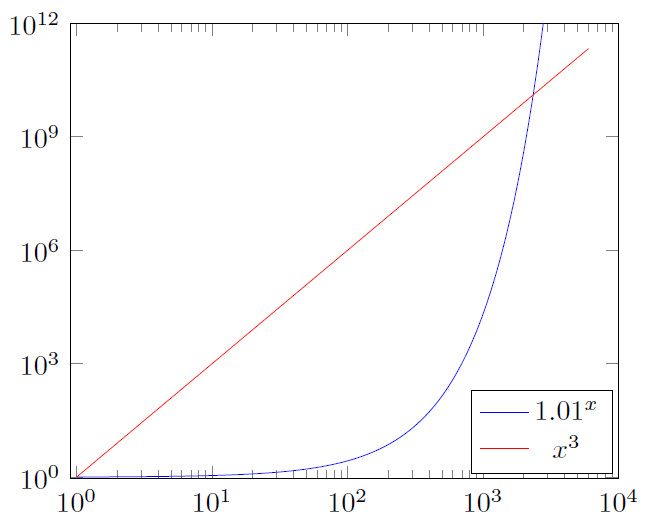
\includegraphics[scale=0.5]{laufzeit/polyVsExp}
\end{frame}

\begin{frame}[t]{Wahr oder Falsch?}
	\TrueQuestionE{$x^4 \in \Oh{{(x^3)}^3}$}{ $ {(x^3)}^3 = x^9$}
	\FalseQuestionE{$\sqrt{n} \in \Om{2^n}$}{}
	\TrueQuestionE{$log_{5000} n \in \Th{\log_2{n^4}}$}{ $ \log_2{n^4} = 4 \cdot \log_2{n}$}
	\FalseQuestionE{$O(f_1) + f_2 = O(f_1 + f_2)$}{Z.~B.: \\ $\Oh{n} + 4 = \set{f(n) + 4 \Mid f(n) \in \Oh{n}} \neq \set{f(n) \Mid f(n) \in \Oh{n}} = \Oh{n+4}$. \\ \textbf{Aber} es gilt: $O(f_1) + O(f_2) = O(f_1 + f_2)$}
\end{frame}

\begin{frame}[t]{Wahr oder Falsch?}
	\FalseQuestion{Für zwei Funktionen $f, g$ gilt immer $f \preceq g$ oder $f \succeq g$.}
	\medskip
	
	\visible<2>{
		Es gibt unvergleichbare Funktionen! Beispiel:
		\begin{align*}
		f(n) &=
		\begin{cases}
		1, & \text{ falls $n$ gerade} \\
		n, & \text{ falls $n$ ungerade} \\
		\end{cases} \\
		g(n) &=
		\begin{cases}
		n, & \text{ falls $n$ gerade} \\
		1, & \text{ falls $n$ ungerade} \\
		\end{cases} \\
		\end{align*}
		Es gilt \textbf{nicht} $g\preceq f$, es gilt \textbf{nicht} $f\preceq
		g$ und es gilt \textbf{erst recht nicht} $f\asymp g$.
	}
\end{frame}


\begin{frame}{Logarithmen encore}
	Berechnet:
	\begin{align*}
	\log_5(25 \cdot 125) &= \visible<2->{\log_5(25) + \log_5(125) = 2+3 = 5}\\
	16^{\log_4(5)} &= \visible<3->{5^{\log_4(16)} = 5^2 = 25}
	\end{align*}
\end{frame}

\begin{frame}{Laufzeiten}
	\pause
	Lineare Suche: \pause $\Th{n}$ \\
	Binäre Suche:  \pause $\Th{\log n}$ \\
	Potenzmenge berechnen: \pause $\Th{2^n}$
\end{frame}

\section{Master-Theorem}

\begin{frame}{Teile und herrsche -- divide and conquer}
	\daniel{Manchmal sind wir zu faul, große Probleme alleine anzupacken...}
	\begin{itemize}
		\item Probleminstanz in kleinere Teile \textbf{zerlegen}
		\item \thassedaniel{Teile rekursiv nach gleichen Verfahren bearbeiten}{Für jeden Teil \textbf{klonen} wir uns einmal und lassen den Klon die Arbeit machen \\
		{\small (Der Klon ist natürlich genauso faul wie wir und klont sich ebenfalls)}}
		\item \thassedaniel{Aus Teilergebnissen Resultat rekonstruieren}{Ergebnisse von den Klonen \textbf{einsammeln} und \textbf{zusammenfügen}}
	\end{itemize}
\end{frame}

\begin{frame}{Das Master-Theorem (einfache Form)}
	Situation aus dem Leben: 
	\begin{itemize}[<+->]
		\item Wir haben einen rekursiven Algorithmus $A$ für ein Problem der Größe $n$
		\item Bei jedem Schritt wird das Problem durch $b$ \textbf{geteilt} und es ergeben sich $d$ neue Probleminstanzen der Größe $n/b$
		\item \thassedaniel{Aufteilen}{Klonen} und Ergebnisse zusammentragen geht in $c \· n$ Operationen (für konstantes $c$)
		%\item Wir können die Laufzeit der jeweiligen \enquote{Auseinandernehmungs-} und \enquote{Zusammenführungsschritte} \textbf{linear} abschätzen.
	\end{itemize}
\end{frame}

\begin{frame}{Das Master-Theorem (einfache Form)}  % TODO Überarbeitung von hier wieder in Algotutfolien übertragen!
	Seien $a, \textcolor{blue}{b}, c, \textcolor{darkgreen}{d}$ positive Konstanten und für $n \in \N$ sei 
	\[
	T(n) = 
	\begin{cases}
	a,  & \text{für } n = 1 \\
	\textcolor{darkgreen}{d} \cdot T\large(\frac{n}{\textcolor{blue}{b}}\large) + c\·n, & \text{für } n > 1
	\end{cases}
	\]
	gegeben. \\ \smallskip
	
	Dann gilt:
	\[
	T(n) \in 
	\begin{cases}
	\Th{n},                                                        & \textcolor{darkgreen}{d} < \textcolor{blue}{b} \\
	\Th{n \log n},                                                 & \textcolor{darkgreen}{d} = \textcolor{blue}{b} \\
	\Th{n^{\log _{\textcolor{blue}{b}} \textcolor{darkgreen}{d}}}, & \textcolor{darkgreen}{d} > \textcolor{blue}{b}
	\end{cases}.
	\]
	%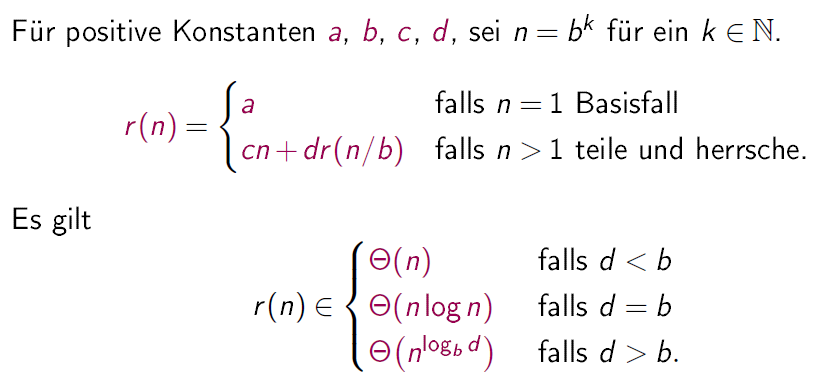
\includegraphics[scale=0.5]{laufzeit/masterTheorem}
\end{frame}

\begin{frame}[t]{MT: Beispiele}
	Wir betrachten verschiedene Sortierverfahren:\\
	\bigskip
	
	\textbf{Mergesort}\\
	msort(L: Liste mit $|L| = n$):\\
	\quad	teile L in der Mitte auf in $L_1$ und $L_2$\\
	\quad	sortiere $L_1$ und $L_2$ mit msort \\
	\quad 	füge $L_1$ und $L_2$ in $\Th{n}$ zusammen\\
	\medskip
	
	$$\text{Laufzeit:} \quad T(n) = \pause \begin{cases}
	1 & n = 1\\
	2 \cdot T(\fract n/2 ) + c \cdot n & n > 1
	\end{cases}$$
	
	\pause
	Nach MT (Fall 2) also: $T(n) \in \Th{n \log n}$.
\end{frame}

\begin{frame}[t]{MT: Beispiele}
	Wir betrachten verschiedene Sortierverfahren:\\
	\bigskip
	
	\textbf{DoubleMergesort}\\
	dmsort(L: Liste mit $|L| = n$):\\
	\quad teile L in der Mitte auf in $L_1$ und $L_2$\\
	\quad sortiere $L_1$ und $L_2$ \textbf{jeweils zwei Mal} mit dmsort\\
	\qquad \textit{Ja, das ist natürlich konstruierter Blödsinn!}\\
	\quad füge $L_1$ und $L_2$ in $\Th{n}$ zusammen\\
	\medskip
	
	$$\text{Laufzeit:} \quad T(n) = \pause \begin{cases}
	1 & n = 1\\
	4 \cdot T(\fract n/2 ) + c \cdot n  & n > 1
	\end{cases}$$
	
	\pause
	Nach MT (Fall 3) also: $T(n) \in \Th{n^{\log_2 4}} = \Th{n^2}$.
\end{frame}

\begin{frame}[t]{MT: Beispiele}
	Wir betrachten verschiedene Sortierverfahren:\\
	\bigskip
	
	\textbf{Magicsort}\\
	magicsort(L: Liste mit $|L| = n$):\\
	\quad teile L in der Mitte auf in $L_1$ und $L_2$\\
	\quad sortiere $L_1$ mit magicsort\\
	\quad sortiere $L_2$ von einem Flaschengeist (in \textbf{Nullkommanichts}!)\\
	\quad füge $L_1$ und $L_2$ in $\Th{n}$ zusammen\\
	\medskip
	
	$$\text{Laufzeit:} \quad T(n) = \pause \begin{cases}
	1 & n = 1\\
	1 \cdot T(\fract n/2 ) + c \cdot n & n > 1
	\end{cases}$$
	
	\pause
	Nach MT (Fall 1) also: $T(n) \in \Th{n}$.
	\medskip
	
	\textbf{ACHTUNG:} Magicsort kann es nicht geben! In Algorithmen I:\\ 
	Untere Schranke für vergleichsbasiertes Sortieren ist $\Om{n \log n}$
\end{frame}


\begin{frame}{Grenzen des MT}
	Nein, das Master-Theorem kann \textbf{nicht} alles (auch wenn es so heißt...). \\
	\smallskip
	\impl Nur verwendbar, wenn die Formeln \textbf{exakt} matchen! (Passiert häufig...) \\
	\smallskip
	In GBI-VL: erweitertes MT (aber auch nicht vollständig!) \\
	\medskip
	Ungleiche Aufteilungen? Vergesst es. \\
	\thasse{Bsp.: \quad Bei der Berechnung von $n! = n \· (n-1)!$ kann die Laufzeit \textbf{nicht} mit dem MT abgeschätzt werden.	}
	
	\mycomment{
		Das Master-Theorem ist mächtig, aber leider längst nicht so mächtig, wie der Name es vielleicht vermuten lässt.\\
		\pause
		Dieses (einfache) MT funktioniert nur bei sehr speziellen Rekurrenzformen (auch wenn diese häufig vorkommen).\\
		\pause
		Ein erweitertes MT wurde in der VL vorgestellt, ist aber auch nicht vollständig!\\
		\pause
		\medskip
		Bei ungleichen Aufteilungen hilft einem das MT überhaupt nicht weiter:\\
		Berechnet man $(n + 1)! = n! \cdot (n + 1)$, so kann die Laufzeit der Berechnung nicht mit dem MT abgeschätzt werden.	
	}
	
	
\end{frame}

\section{Automaten}

\begin{frame}{Endliche Automaten}
	Ein deterministischer endlicher Automat...
	\begin{itemize}
		\item besteht aus endlich vielen Zuständen
		\item ist zu jedem Zeitpunkt in \emph{genau einem} dieser Zustände
		\item wechselt bei Eingabe \emph{genau eines} Zeichens den Zustand in \emph{genau einen, definierten} Folgezustand
		\item und gibt dabei ein Wort als Ausgabe aus
	\end{itemize}

	Die gültigen \enquote{Zustandswechsel} sind als Zustandsübergänge definiert.
\end{frame}

\begin{frame}{Anwendungen}
	\begin{itemize}
		\item Getränkeautomaten
		\item Textsuche
		\item Textersetzung
	\end{itemize}

	Für Beispiele zur Textsuche und Textersetzung: Übung~12, WS~15/16
\end{frame}

\mycomment{ % As a source for copy/pasting:
\begin{tikzpicture}[->,>=stealth,shorten >=1pt,auto,node distance=2.8cm,
semithick,initial text={}]
\tikzstyle{every state}=[fill=red,draw=none,text=white]

\node[initial,state] (A)                    {$q_a$};
\node[state]         (B) [above right of=A] {$q_b$};
\node[state]         (D) [below right of=A] {$q_d$};
\node[state]         (C) [below right of=B] {$q_c$};
\node[state]         (E) [below of=D]       {$q_e$};

\path (A) edge              node {0,1,L} (B)
		  edge              node {1,1,R} (C)
(B) edge [loop above] node {1,1,L} (B)
	edge              node {0,1,L} (C)
(C) edge              node {0,1,L} (D)
	edge [bend left]  node {1,0,R} (E)
(D) edge [loop below] node {1,1,R} (D)
	edge              node {0,1,R} (A)
(E) edge [bend left]  node {1,0,R} (A);
\end{tikzpicture}	
}

\subsection{Mealy-Automaten}
\begin{frame}{Ein einfacher Automat}
	\begin{center}
		\begin{tikzpicture}[->,>=stealth,shorten >=1pt,auto,node distance=2.8cm,
			semithick,initial text={}]
			\tikzstyle{every state}=[]
			
			\node[initial,state] (A)                    {$a$};
			\node[state]         (M) [right of=A] 	    {$m$};
			
			\path (A) edge [loop above] node {\word 1|\word 0} (A)
			          edge [loop below]  node {\word 0|\word 1} (A)
			          edge 					  node {\word{2}|\word{X}} (M)
			      (M) edge [loop right] node {$\stackedtight{\word 0|\word X \\ \word 1|\word X \\ \word 2|\word X}$} (M);
			      %(M) edge [loop right] node {\word 1|\word X} (M)
			      %(M) edge [loop below] node {\word 2|\word X} (M);
		\end{tikzpicture}
	\end{center}
	\pause
	Eingabe: \word{011101} \?> Ausgabe: \word{100010} \\
	Eingabe: \word{011102} \?> Ausgabe: \word{10001X} \\
	Eingabe: \word{012101} \?> Ausgabe: \word{10XXXX} \\ \pause
	\smallskip
	\impl Der Automat negiert das Eingabewort bitweise. \\
	(Frisst er ne \word 2, so isser beleidigt. \smiley)
\end{frame}

\begin{frame}{Mealy-Automat}
	Bei einem Mealy-Automaten findet die Ausgabe \textbf{bei den Zustandsübergängen} statt.
	\begin{Definition}
		Ein \textbf{Mealy-Automat} $ A = (Z,z_0,X,f,Y,g)$ besteht aus...
		\begin{itemize}
			\item einer endlichen Zustandsmenge $Z$ 
			\item einem Startzustand $z_0$
			\item einem Eingabealphabet $X$ 
			\item einer Zustandsübergangsfunktion $f \from Z\times X \functionto Z $
			\item einem Ausgabealphabet $Y$
			\item einer Ausgabefunktion $g \from Z\times X \functionto Y^* $ 
		\end{itemize}						
	\end{Definition}
\end{frame}

\begin{frame}{}
	\begin{block}{Graphische Darstellung}
		\begin{itemize}
			\item Oft malt man Automaten hin. (Achtung: Die formale Schreibweise wird trotzdem auch im Studium verwendet! Also auswendig lernen!)
			\item Zustände sind \textbf{Knoten} und Übergänge sind \textbf{gerichtete Kanten} in einem Graphen. \\
			Kanten\textbf{beschriftung}: „$\langle\text{Eingabe}\rangle | \langle\text{Ausgabe}\rangle$“
			\item \textbf{Der Startzustand wird mit einem Pfeil \enquote{aus dem Nichts} gekennzeichnet!}  \pause
			\implitem \textbf{NICHT VERGESSEN!} Kostet sonst Punkte! \textbf{Immer!}
		\end{itemize}
		
	\end{block}
\end{frame}

\begin{frame}{Beispiel: Automatengraphen}
	%\vspace{-1\baselineskip} 
	%\hspace{-\baselineskip}
	
\includegraphics[page=3,trim=18px 47px 18px 14px,clip]{U12.pdf}	
\end{frame}

%% Übung: Beispiel
%\setbeamercolor{background canvas}{bg=}


\begin{frame}{Eingabe eines Zeichens}
	Was ist die Zustandsübergangsfunktion $f$? \\ \pause
	\medskip
	Haben
	\begin{itemize}
		\item aktuellen Zustand $z \in Z$
		\item eingelesenes Zeichen $x \in X$
	\end{itemize}
	\impl $f$ liefert den Folgezustand $z_\text{neu}$, in welchem der Automat danach ist.\\
	\medskip
	Formell: $$ f(z,x) = z_\text{neu} $$ 
\end{frame}

\begin{frame}{Eingabe eines Wortes}
	Was machen wir mit ganzen Wörtern? \\ \pause
	Wir definieren uns ganz analog
	\begin{block}{Zustandsübergangsfunktion extended}
	\begin{align*}
		 	f_*(z,\eps) &:= z \\
		 	\forall w\in X^* , \, x\in X : \quad  f_*(z,wx) &:= f\left(f_*(z,w),x\right) 
	\end{align*}
	\end{block}
	\pause Was macht diese Funktion? \\ \pause
	\medskip
	Haben
	\begin{itemize}
		\item aktuellen Zustand $z \in Z$
		\item eingelesenes Wort $w \in X^*$
	\end{itemize}
	\impl $f_*$ liefert den \textbf{Endzustand} $z_\text{ende}$, in welchem der Automat \textbf{nach dem Wort} dann ist.
	Formell: $$ f_*(z,w) = z_\text{ende} $$
	%Bei Eingabe eines Wortes $w$ und Anfangszustand $z$ gibt sie den Zustand $z' = f_*(z,w)$ aus, in dem der Automat enden wird. 
\end{frame}
	
\begin{frame}{Eingabe eines Wortes}
	Definieren wir nun weiter 
	\begin{block}{Zustandsübergangsfunktion extended extended}
		\begin{align*}
			f_{**}(z, \eps) &:= z \\
			\forall w\in X^* , \, x\in X : \quad  f_{**}(z, xw)   &:= z \cdot f_{**}\!\left(f(z,x),w\right) \\
		\end{align*}
	\end{block}
	\pause Was macht diese Funktion? \\ \pause
	Diese Funktion gibt die Reihe aller \textbf{Zustände als Gesamtwort} aus, die der Automat bei Eingabe des Wortes $w$ im Startzustand $z$ durchläuft. Also: 
	$$ f_{**}(z, w) = z \* z_1 \* z_2 \cdots z_\text{ende} $$
\end{frame}

\begin{frame}{Eingabe eines Wortes}		
	Alternative Definition:
	\begin{block}{Zustandsübergangsfunktion extended extended}
		\begin{align*}
			f_{**}(z,\varepsilon) &= z \\
			\forall w \in X^* \ \forall x \in X : f_{**}(z,wx) &= f_{**}(z,w)\cdot f(f_*(z,w),x)	 
		\end{align*}
	\end{block}
\end{frame}

\begin{frame}{Beispiel $f, f_*, f_{**}$}
	\begin{center}
			\begin{tikzpicture}[->,>=stealth,shorten >=1pt,auto,node distance=2.8cm,
		semithick,initial text={}]
		\tikzstyle{every state}=[]
		
		\node[initial,state] (A)                    {$a$};
		\node[state]         (M) [right of=A] 	    {$m$};
		
		\path (A) edge [loop above] node {\word 1|\word 0} (A)
		edge [loop below]  node {\word 0|\word 1} (A)
		edge 					  node {\word{2}|\word{X}} (M)
		(M) edge [loop right] node {$\stackedtight{\word 0|\word X \\ \word 1|\word X \\ \word 2|\word X}$} (M);
		\end{tikzpicture}
	\end{center}
	\begin{align*}
		f(a, \word 2) &= m \\
		f(a, \word 0) &= a \\ 
	\end{align*}
	\pause  \vspace{-2.5\baselineskip}
	\begin{align*}
		f_*(a, \word{101}) &= \hphantom{aa}a \\
		f_{**}(a, \word{101}) &= aaa \\ 
	\end{align*}
	\pause  \vspace{-2.5\baselineskip}
	\begin{align*}
		f_*(a, \word{1021}) &= \hphantom{aam}m \\
		f_{**}(a, \word{1021}) &= aamm
	\end{align*}
\end{frame}

\begin{frame}{Ausgaben}
	Automaten können ja was ausgeben. \\
	\smallskip
	Erinnerung: Die Kanten sind beschriftet mit $x \mid y$ , wobei $x\in X$ und $y\in Y^* $. \\
	 \impl Für Eingabe $x$ wird das Wort $y$ ausgegeben. \\ 
	Formal: $$g(z,x) = y$$
\end{frame}

\begin{frame}{Ausgabefunktionen}
	\begin{block}{Ausgabefunktion extended}
		Wir können also analog zu $f_*$ und $f_{**}$ definieren
		\begin{threealign}
		\text{Für die letze Ausgabe: } \qquad g_* : Z\times X^* &\functionto& Y^* \\
		g_*(z,\varepsilon) &=& \varepsilon \\
		\forall w\in X^* \; \forall x\in X : g_*(z,wx) &=& g(f_*(z,w),x) \\ \\
		\text{Für das ganze Ausgabewort: } \qquad g_{**} : Z\times X^* &\functionto& Y^* \\ 
		g_{**}(z,\varepsilon) &=& \varepsilon \\
		\forall w\in X^* \; \forall x\in X : g_{**}(z,wx) &=& g_{**}(z,w)\cdot g_*(z,wx) 			
		\end{threealign} 
	\end{block}
	
	%\pause Dies gibt nun nicht die durchlaufenen Zustände bzw. den Abschlusszustand an, sondern die letzte Ausgabe bzw. alle durchlaufenen Ausgaben. 

\end{frame}

\begin{frame}{Beispiel $g, g_*, g_{**}$}
	\begin{center}
		\begin{tikzpicture}[->,>=stealth,shorten >=1pt,auto,node distance=2.8cm,
		semithick,initial text={}]
		\tikzstyle{every state}=[]
		
		\node[initial,state] (A)                    {$a$};
		\node[state]         (M) [right of=A] 	    {$m$};
		
		\path (A) edge [loop above] node {\word 1|\word 0} (A)
		edge [loop below]  node {\word 0|\word 1} (A)
		edge 					  node {\word{2}|\word{X}} (M)
		(M) edge [loop right] node {$\stackedtight{\word 0|\word X \\ \word 1|\word X \\ \word 2|\word X}$} (M);
		\end{tikzpicture}
	\end{center}
	\vspace{-\baselineskip}
	\begin{align*}
	g(a, \word 2) &= \word X \\
	g(a, \word 0) &= \word 1 \\ 
	\end{align*}
	\pause  \vspace{-2.5\baselineskip}
	\begin{align*}
	g_*(a, \word{101}) &= \hphantom{\word{01}}\word 0 \\
	g_{**}(a, \word{101}) &= \word{010} \\ 
	\end{align*}
	\pause  \vspace{-2.5\baselineskip}
	\begin{align*}
	g_*(a, \word{1021}) &= \hphantom{\word{01X}}\word X \\
	g_{**}(a, \word{1021}) &= \word{01XX} \\ 	\visible<+->{}
	\visible<+->{g_*(m, \word{0110}) &= }\visible<+->{\word X}
	\end{align*}
\end{frame}


\subsection{Moore-Automat}
\begin{frame}{Moore-Automat}
	Moore-Automaten sind fast genauso aufgebaut wie Mealy-Automaten.\\ \smallskip
	\textbf{Unterschied}: Ausgabe erfolgt „\textbf{im Zustand}“, nicht beim Zustandsübergang. \\ \pause 
	\begin{tabular}{cc}
		Mealy: & Moore: \\
		\begin{tikzpicture}[->,>=stealth,shorten >=1pt,auto,node distance=2.8cm,
		semithick,initial text={}]
		\tikzstyle{every state}=[]
		
		\node[state,white] (X)                    {\hphantom{XXX}};
		\node[state]         (A) [right of=X] 	    {$A$};
		
		\path (X) edge [bend left=9]	 node {\word a|\word 0} (A)
				  edge [bend right=9]	 node [below] {\word b|\word 1} (A);
		\end{tikzpicture}
		&
		\begin{tikzpicture}[->,>=stealth,shorten >=1pt,auto,node distance=2.8cm,
		semithick,initial text={}]
		\tikzstyle{every state}=[]
		
		\node[state,white] (X)                    {\hphantom{XXX}};
		\node[state]         (A) [right of=X] 	    {$A|\word{XY}$};
		
		\path (X) edge [bend left=9]	 node {\word a } (A)
				  edge [bend right=9]	 node [below] {\word b } (A);
		\end{tikzpicture}
	\end{tabular} \\
	\pause
	Ausgabefunktion heißt jetzt also auch: $$h\from Z\functionto Y^*$$ \impl Ausgabe hängt \textbf{nicht} von der Eingabe ab!\\
\end{frame}

\begin{frame}{Moore-Automat – Ausgabe}
	Ausgabefunktion heißt jetzt also auch: $$h\from Z\functionto Y^*$$ \impl Ausgabe hängt \textbf{nicht} von der Eingabe ab!\\ 
	Dann def. wir $$ g_* (z,w) := h(f_*(z,w)) $$
	\pause
	Für $g_{**}$ gilt dann mit $h^{**}\from Z^*\functionto Y^*$ \quad (der durch $h$ induzierte Hom.!)  $$ g_{**}(z,w) = h^{**} (f_{**}(z,w)) $$
	Wir wenden also $h$ auf jeden durchlaufenen Zustand an.
\end{frame}


\begin{frame}{Beispiel Moore-Automat}
	
\includegraphics[page=11,trim=18px 47px 18px 13px,clip]{U12.pdf}	
\end{frame}


\begin{frame}{Umwandlung von Automaten: Moore $\leftrightsquigarrow$ Mealy}
	\begin{block}{Von Moore zu Mealy}
		Relativ straightforward.\\
		Ausgaben \enquote{aus den Knoten auf die Übergänge ziehen}\\
		\medskip
		\textbf{Beachte}: Für die Eingabe $\eps$ kann ein Moore-Automat eine Ausgabe $g_{**}(s, \eps) \neq \eps$ erzeugen, ein Mealy-Automat \emph{jedoch nicht}.
	\end{block}

	\begin{block}{Von Mealy zu Moore}
		Komplizierter
	\end{block}
\end{frame}



\begin{frame}{Beispiel: Umwandlung von Mealy nach Moore}
	%\vspace{-2\baselineskip}
	\begin{tikzpicture}[->,>=stealth,shorten >=1pt,auto,node distance=2.8cm,
	semithick,initial text={}]
	\tikzstyle{every state}=[]
	
	\node[initial,state] (A)                    {$a$};
	\node[state]         (M) [right of=A] 	    {$m$};
	
	\path (A) edge [loop above] node {\word 1|\word 0} (A)
	edge [loop below]  node {\word 0|\word 1} (A)
	edge 					  node {\word{2}|\word{X}} (M)
	(M) edge [loop right] node {$\stackedtight{\word 0|\word X \\ \word 1|\word X \\ \word 2|\word X}$} (M);
	\end{tikzpicture}
	\\
	\pause  
	\vspace{-1\baselineskip}
	%\hspace{.6\textwidth} 
	\begin{tikzpicture}[->,>=stealth,shorten >=1pt,auto,node distance=2.1cm,
	semithick,initial text={}]
	\tikzstyle{every state}=[]
	
	\node[initial,state] (A)                    {$a|\eps$};
	\node[state]         (B) [above right of=A] 	    {$b|\word 0$};
	\node[state]         (C) [below right of=A] 	    {$c|\word 1$};
	\node[state]         (M) [below right of=B] 	    {$m|\word X$};
	
	\path 
		(A) edge 				node {\word 1} (B)
		(A) edge 				node [below] {\word 0} (C)
		(B) edge [bend left=8]	node {\word 0} (C)
		(C) edge [bend left=8]	node {\word 1} (B)
		(B) edge 				node {\word 2} (M)
		(C) edge 				node [below] {\word 2} (M)
		(M) edge [loop right]	node {\word 0, \word 1, \word 2} (M)
	;
	\draw[->] (A) to[out=-90,in=-90, looseness=1.87] (M) node [at start, below=55pt, right=4pt] {\word 2}; %Fuck you, LaTeX. "midway" node option doesn't work at all.
	\end{tikzpicture}
\end{frame}

\only<beamer:0>{

\begin{headframe}[\daniel{Zu hässlich zum Wegwerfen}]
	Unübersichtliche Beispiele
\end{headframe}

\begin{frame}{Beispiel: Ein Getränkeautomat}
	$\word R$ sei reines Wasser, $\word Z$ ist Zitronenlimonade, $\word O$ ist OK (Getränkeausgabe), $\word C$ ist Clear und $\word 1$ entspricht einer 1-€-Münze. (\word - heißt „kein Getränk ausgewählt“)\\
	Wir wollen: \pause
	\begin{itemize}[<+->]
		\item Getränk wählen können
		\item Geld rein- und rausholen können
		\item und immer zurück kommen können! ($=$ Abbruch-Knopf)
	\end{itemize}
\end{frame}

\begin{frame}
	\begin{figure}[H]
		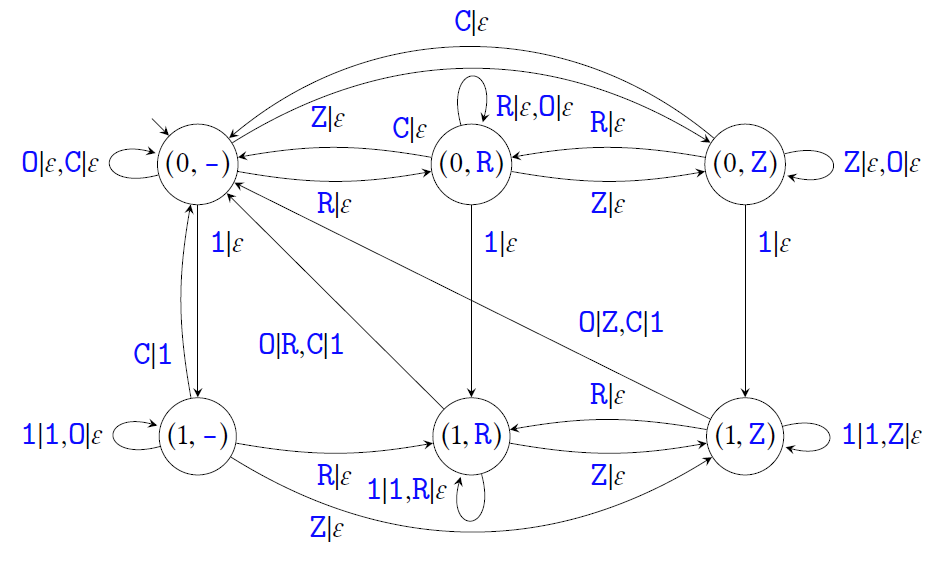
\includegraphics[scale=0.4]{automaten/getraenke} % ist „ohne Ausgabe“ überhaupt erlaubt?? Ich denke nicht.
	\end{figure}
	
	Was ist $f((0,\word -), \word Z), \, f_*((0,\word -), \word{R10}) ,  \, f_{**}( (0,\word -),\word{R10}) $ ? Rechnerisch und graphisch.	
	
\end{frame}

\begin{frame}
	Rechnerisch nur der 3. Fall:
	\begin{threealign}
	f_{**}((0,\word -),\word{R10}) &=& f_{**}((0,\word -),\word{R1}) )\cdot f(f_*((0,\word -),\word{R1}),\word{0}) \\ 
	&=& f_{**} ((0,\word -),\word R) \cdot f(f_*((0,\word -),\word R),\word 1) \\& & \mbox{} \cdot f(f_*((0,\word -),\word{R1}),\word 0) \\ 
	&=& f_{**}((0,\word -),\eps) \cdot f(f_*((0,\word -),\eps),\word R) \\ &&\mbox{} \cdot f(f_*((0,\word -),\word R),\word 1) \cdot f(f_*((0,\word -),\word{R1}),\word 0) \\ 
	&=& (0,\word -) \cdot f((0,\word -),\word R) \cdot f( f(f_*((0,\word -),\eps),\word R),\word 1) \\ &&\mbox{} \cdot f( f(f_*((0,\word -),\word R),\word 1),\word 0) \\
	&=& (0,\word -) \cdot f((0,\word -),\word R) \cdot f( f((0,\word -),\word R),\word 1)  \\& &\mbox{} \cdot f(f(  f(f_*(0,\word -),\eps),\word R),\word 1), \word 0) \\
	&=& (0,\word -) \cdot f((0,\word -),\word R) \cdot f( f((0,\word -),\word R),\word 1)\\ &&\mbox{} \cdot f( f(f((0,\word -),\word R),\word 1),\word 0) \\ 
	&=& (0,\word -) \cdot (0,\word R) \cdot (1,\word R) \cdot (0,\word -) 
	\end{threealign} 
\end{frame}

\begin{frame}{Beispiel}
	\begin{figure}[H]
		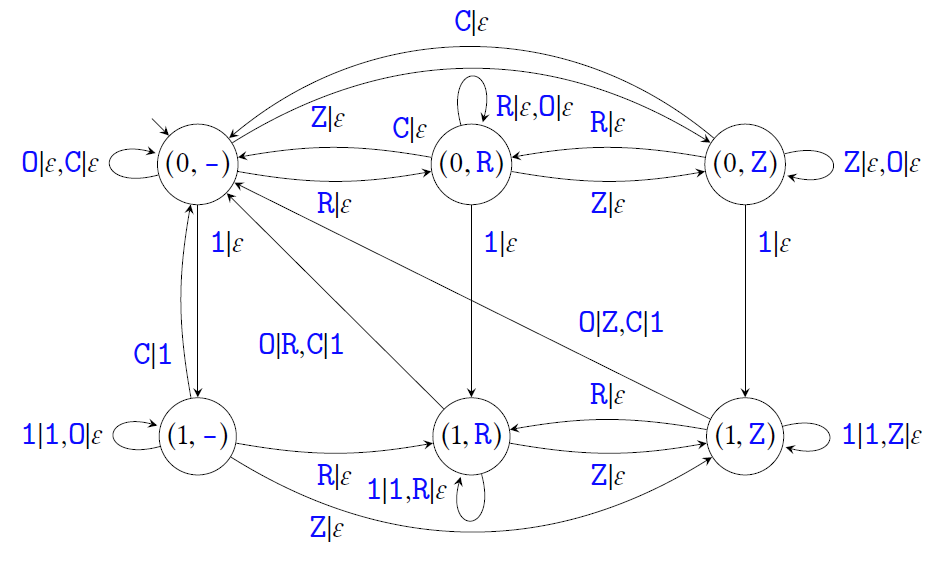
\includegraphics[scale=0.4]{automaten/getraenke}			
	\end{figure}
	Was ist $g_*((0,\word -), \word{R10}) , \, g_{**}((0,\word -),\word{R10}) , \, g_{**}((0,\word -),\word{R110}) $ ? \\ \pause
	$g_*((0,\word -),\word{R10}) = g_{**}((0,\word -),\word{R10}) = \word R, \qquad g_{**}((0,\word -),\word{R110}) = \word{1R} $	
\end{frame}

\begin{frame}{}
	Beispiel: Automaten-Umwandlung (Übung 12, WS 15/16)
\end{frame}

%% Übung: Beispiel
\setbeamercolor{background canvas}{bg=}

\includepdf[pages={34-40}]{U12.pdf}
}

\section{Endliche Akzeptoren}
\begin{frame}[t]{Endliche Akzeptoren}
	\begin{Definition}
		Ein \textbf{endlicher Akzeptor} $A$ ist ein \emph{Moore}-Automat mit Ausgabealphabet $ Y= \{\word 0,\word 1\}$, der zuletzt $\word 1$ ausgibt, falls ihm das Wort gefällt und \word 0 sonst. %, falls das eingegebene Wort der vorliegenden Syntax entspricht und $0$ sonst.
	\end{Definition} 
	
	$A$ \textbf{akzeptiert} ein Wort $w$, wenn er als Letztes eine $\word 1$ ausgibt. \\ \medskip 
	
	\only<all:2>{
		\begin{center}
					\begin{tikzpicture}[->,>=stealth,shorten >=1pt,auto,node distance=1.8cm,
				semithick,initial text={}]
				\tikzstyle{every state}=[]
				
				\node[state] (A)                    {$a|\word 0$};
				\node[state] (B) [right of=A] 	    {$b|\word 1$};
				
				\end{tikzpicture}
		\end{center}
	}
	\only<all:3>{
		\begin{center}
					\begin{tikzpicture}[->,>=stealth,shorten >=1pt,auto,node distance=1.8cm,
				semithick,initial text={}]
				\tikzstyle{every state}=[]
				
				\node[state] (A)                    {$a$};
				\node[state, accepting] (B) [right of=A] {$b$};
				
				\end{tikzpicture}
		\end{center} 
		\emph{Notation:} Wir nennen die Menge der \textbf{akzeptierenden Zustände} $F$ und malen solche mit einem Doppelkreis. \\ 
	}
\end{frame}

\begin{frame}{Von einem Akzeptor erkannte Sprache}
	Wir sprechen von einer \textbf{akzeptierten Sprache} über einem Alphabet. Sie ist definiert als 
	\begin{align*}
		L(A) &:= \{ w \mid f_*(z_0,w) \in F \}  \\
			 &\: = \{ w \mid g_*(z_0,w) = \word 1 \}.
	\end{align*}
	Also sind in einer akzeptierten Sprache alle Wörter, die von $A$ akzeptiert werden. \pause
	
	\begin{Beispiel}
		Sei $A$ gegeben als
		\vspace{-2\baselineskip}
		\begin{center}
			\begin{tikzpicture}[->,>=stealth,shorten >=1pt,auto,node distance=1.8cm,
			semithick,initial text={}]
			\tikzstyle{every state}=[]
			
			\node[initial, state, accepting] (A)                    {$0$};
			\node[state] (B) [right of=A] {$1$};
			
			\path
				(A) edge [loop above] node {\word a,\word b}  (A)
					edge [bend right=7] node [below] {\word c} 		  (B)
				(B) edge [loop right] node {\word c}		  (B)
					edge [bend right=7] node [above] {\word a, \word b} (A)
			;
			\end{tikzpicture}. % Sätze enden mit nem Punkt! :D
		\end{center} 
		\pause
		Dann ist $L(A) = \set{w \in \set{\word a, \word b, \word c} \Mid \text{$w$ endet nicht auf \word c}}$.
	\end{Beispiel}
\end{frame}

% DJ: Furchtbares Beispiel. Viel zu fett.
%% Übung: Beispiel  
%\setbeamercolor{background canvas}{bg=}
%
\includepdf[pages=44]{U12.pdf}

\begin{frame}{Aufgaben}
	Gebt einen Akzeptor an, der die Sprache aller Binärzahlen erkennt, die Zweierpotenzen darstellen. 
	\pause ($= \set{\word 0}^* \· \set{\word 1} \· \set{\word 0}^*$) \\
	%\vspace{-2\baselineskip}
	\begin{center}
		\begin{tikzpicture}[->,>=stealth,shorten >=1pt,auto,node distance=2cm,
		semithick,initial text={}]
		\tikzstyle{every state}=[]
		
		\node[initial,state] (A)                    {$a$};
		\node[state,accepting] (B)  [right of=A]     {$b$};
		\node[state]		 (M)  [right of=B]		{$m$};
		
		\path
		(A) edge [loop above]  node {\word 0} (A) 
		(A) edge 			  node {\word 1} (B) 
		(B) edge [loop above]  node {\word 0} (B) 
		(B) edge 			  node {\word 1} (M) 
		(M) edge [loop above] node {\word 0, \word 1} (M);
		\end{tikzpicture}
	\end{center}
	\pause
	Gebt einen Akzeptor an, der die Sprache aller geraden Binärzahlen erkennt. 
	\pause ($= \set{\word 0,\word 1}^* \· \set{\word 0}^+$) \\
	%\vspace{-2\baselineskip}
	\begin{center}
		\begin{tikzpicture}[->,>=stealth,shorten >=1pt,auto,node distance=1.8cm,
		semithick,initial text={}]
		\tikzstyle{every state}=[]
		
		\node[initial, state] (A)                    {$a$};
		\node[state, accepting] (B) [right of=A] {$b$};
		
		\path
		(B) edge [loop above] node  {\word 0}  (B)
			edge [bend right=7] node [above] {\word 1} 		  (A)
		(A) edge [loop above] node  {\word 1}		  (A)
			edge [bend right=7] node [below] {\word 0} (B)
		;
		\end{tikzpicture}
	\end{center} 
\end{frame}

\begin{frame}{Aufgabe}
	Der endliche Akzeptor $A = (Z, z_0, X, f, F)$ sei gegeben durch
	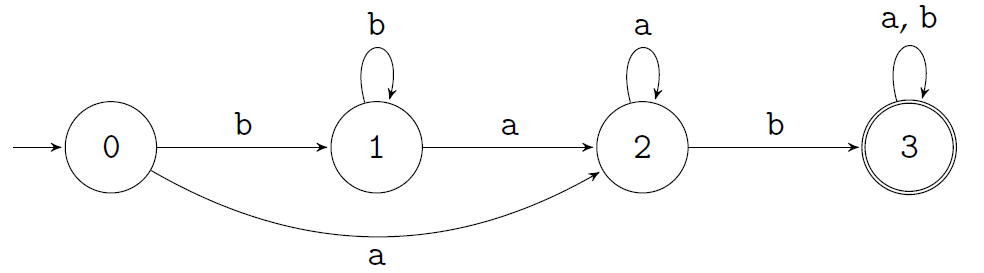
\includegraphics[scale=0.4]{automaten/akz1516B12A1}
	
	Gebt die von $A$ akzeptierte Sprache $L(A)$, unter ausschließlicher Benutzung der formalen Sprachen $\{\word a\}$, $\{\word b\}$, sowie $\{\word a, \word b\}$, des Konkatenationsabschlusses und des Produkts formaler Sprachen, an.
	
	\emph{Beispiel:} $\{\word a, \word b\}^* \cdot \{\word a\} \cdot \{\word b\}$
	
	\visible<2-|handout:2>{
		\begin{block}{Lösung}
			$L(A) = \{\word b\}^* \cdot \{\word a\} \cdot \{\word a\}^* \cdot \{\word b\} \cdot \{\word a, \word b\}^*$ \\
			$\hphantom{L(A) } = \{\word b\}^* \cdot \hphantom{\{\word a\} \cdot \mbox{}} \{\word a\}^+ \!\cdot \{\word b\} \cdot \{\word a, \word b\}^*$
		\end{block}
	}
\end{frame}

\begin{frame}{Aufgabe}
	\begin{enumerate}[a)]
		\item Zeichnet einen möglichst kleinen endlichen Akzeptor mit $ X = \{\word a, \word b\}$, der alle Wörter akzeptiert, bei denen die Anzahl der $\word a$ durch $5$ teilbar ist.
		\item Zeichnet einen Akzeptor mit $ X = \{\word a,\word b\}$, der alle Wörter akzeptiert, in denen nirgends hintereinander zwei $\word b$ vorkommen.
	\end{enumerate}		
\end{frame}

\begin{frame} {Lösung a)}
	\begin{figure}[H] 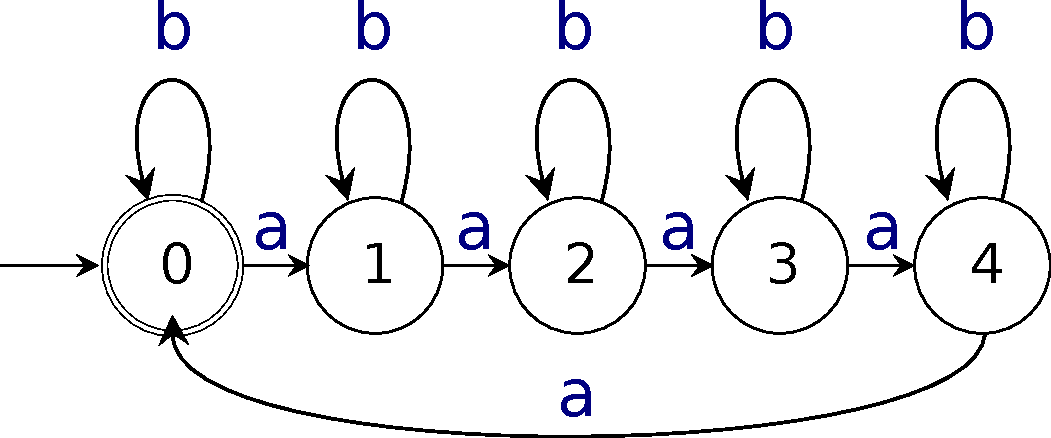
\includegraphics[scale=0.5]{automaten/Akzeptor1.pdf} \end{figure}		
\end{frame} 

\begin{frame}{Lösung b)}
	\begin{figure}[H] 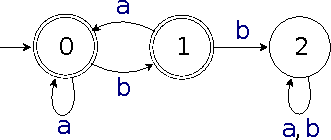
\includegraphics[scale=1.5]{automaten/Akzeptor2.pdf} \end{figure}
\end{frame}



% ---------

% WiSe 10/11 Aufgabe 6 c 
\begin{frame}{Übung: Akzeptoren}
	Die Sprache $L\subseteq \{\word a,\word b\}^\ast $ sei definiert als die Menge aller Wörter $w$, die folgende Bedingungen erfüllen:
	\begin{align*}
		N_{\word b}(w) &> N_{\word a}(w)\\ 
		\forall v_1,v_2 \in \{\word a,\word b\}^\ast : \qquad w &\neq v_1 \word{bb} v_2 
	\end{align*}
	
	Gebt einen endlichen Akzeptor an, der $L$ erkennt. \\
	
	\bigskip
	\pause
	\begin{block}{Tipps}
		\begin{itemize}[<+->]
			\item Die zweite Bedingung bedeutet: Das Wort darf nirgends zwei \word b hintereinander enthalten.
			\item Was passiert, wenn das Wort mit einem \word a beginnt?\\
				  Kann das Wort noch akzeptiert werden?
		\end{itemize}
	\end{block}
\end{frame}

\begin{frame}{Übung: Akzeptoren: Lösung}
	\begin{figure}
		\centering
		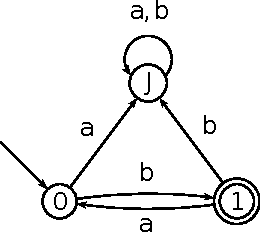
\includegraphics[width=0.7\linewidth]{automaten/Loesung2.pdf}
	\end{figure}
\end{frame}

% TODO: Fix dirty hack in thwregex.sty, where I changed line 42 to print star in math-mode
% 		because otherwise the star was always raised in my config.
%		Use \rx everywhere

% This slide is only here because \only dosn't work in Title
\ifdefined \handout \else
\begin{frame}{}
	Gibt es einen endlichen Akzeptor mit $$L = \{ a^kb^k | k\in \N_0 \}$$
	% This is to reserve the space so the text doesn't jump
	\visible<0>{Nein! Warum nicht?\\
		
		Gibt es einen endlichen Akzeptor, der alle gültigen Klammerausdrücke erkennt?\\
		Nein, aus dem selben Grund.
		\begin{figure}[H]
			
\includegraphics[scale=0.5]{xkcd/tags_1144}
			\caption{ \texttt{\url{https://www.xkcd.com/1144/}} }
		\end{figure}
		Kontextfreie Grammatiken \enquote{können also mehr} als endliche Automaten.\\
		Wir wollen nun ein \enquote{gleichmächtiges} Konzept.}
\end{frame}
\fi

\begin{frame}{Grenzen endlicher Automaten}
	Gibt es einen endlichen Akzeptor mit $$L = \{ a^kb^k | k\in \N_0 \}$$
	Nein! Warum nicht?\\
	
	Gibt es einen endlichen Akzeptor, der alle gültigen Klammerausdrücke erkennt?\\ \pause
	Nein, aus dem selben Grund.
	\begin{figure}[H]
		
\includegraphics[scale=0.5]{xkcd/tags_1144}
		\caption{ \texttt{\url{https://www.xkcd.com/1144/}} }
	\end{figure}
	\pause
	Kontextfreie Grammatiken \enquote{können also mehr} als endliche Automaten.\\
	Wir wollen nun ein \enquote{gleichmächtiges} Konzept.
\end{frame}

\section{Reguläre Ausdrücke}
\subsection{Definition}

\begin{frame}{Reguläre Ausdrücke}
	Wir können uns reguläre Ausdrücke zusammenbauen aus
	\begin{itemize}[<+->]
		\item den einzelnen Symbolen $x$ aus $A$
		\item zwei regulären Ausdrücken $R_1$ und $R_2$ mit $$(R_1 R_2) \qquad \text{ oder } \qquad (R_1 \mid R_2)$$
		\item einem Stern $R\ast$
		\item oder dem leeren Ausdruck
	\end{itemize} \pause
	Klammern dürfen nach den Klammerregeln weggelassen werden:\\
	Stern vor Punkt vor Strich.
\end{frame}

\begin{frame}{Reguläre Ausdrücke}
	\begin{Beispiel}
		Sei $ A = \{ a, b, c\}$. Dann sind gültige reguläre Ausdrücke:\\
		$\rx{abc}$\\
		$\rx{a|b|c}$\\
		$\rx{(ab)*}$\\
		$\rx{O*}$
	\end{Beispiel}
\end{frame}


\begin{frame}{Sprache eines Ausdruckes}
	Die durch $R$ beschriebene Sprache $\lang{R}$ ist wie folgt definiert:
	\begin{itemize}
		\item $\lang{\rx{O}} = \emptyset$
		\item $\lang{x}=\{x\} \; (x\in A)$
		\item $\lang{R_1 \rx| R_2} = \lang{R_1} \cup \lang{R_2}$
		\item $\lang{R_1 R_2} = \lang{R_1} \cdot \lang{R_2}$
		\item $\lang{R\rx*} = \lang{R}^*$
	\end{itemize} 
\end{frame}

\begin{frame}
	\begin{Beispiel}
		\begin{itemize}[<+->]
			\item $\lang{\rx{a}} = \{\#a\}$
			\item $\lang{\rx{ab}} = \lang{\rx{a}} \cdot \lang{\rx{b}} = \{\#a\#b\}$
			\item $\lang{\rx{a|b}} = \lang{\rx{a}}\cup\lang{\rx{b}} = \{\#a,\#b\}$.
			\item $\lang{\rx{(a|b)*}} = \lang{\rx{a|b}}^* = \{\#a,\#b\}^*$.
			\item $\lang{\rx{(a*b*)*}} = \lang{\rx{a*b*}}^* = (\lang{\rx{a*}}\lang{\rx{b*}})^* 
			= (\lang{\#a}^*\lang{\#b}^*)^* = (\{\#a\}^*\{\#b\}^*)^*$\\
			$= \{\#a,\#b\}^*$. 
		\end{itemize}
	\end{Beispiel}
\end{frame}

\begin{frame}{Aufgabe: Reguläre Ausdrücke}
	In dieser Aufgabe geht um die formalen Sprachen
	$$L_1 = \{a^k b^m \mid k, m \in \N_0 \} \qquad L_2 = \{b^k a^m \mid k, m \in \N_0 \}$$
	Geben Sie für jede der folgenden formalen Sprachen $L$ je einen regulären Ausdruck $R$ an mit $ \langle R \rangle = L$.
	\begin{itemize}
		\item $L = L_1 \cup L_2$ 
			\only<2-|handout:2>{$\qquad a\ast b\ast \mid b\ast a\ast$}
		\item $L = L_1 \cap L_2$
			\only<3-|handout:2>{$\qquad a\ast \mid b\ast $}
		\item $L = L_1\cdot L_2$
			\only<4-|handout:2>{$\qquad a\ast b\ast b\ast a\ast$ oder $a\ast b\ast a\ast$}
		\item $L = L_1\ast$
			\only<5-|handout:2>{$\qquad (a\ast b\ast)\ast$ oder $(a\mid b)\ast$}
	\end{itemize}
\end{frame}

\begin{frame}{Aufgabe: Sprachen regulärer Ausdrücke}
	\begin{itemize}
		\item $\lang{\rx{(a|b)*abb(a|b)*}} =$
		\item $\lang{\rx{a**}} $
		\item $\lang{???} = \lang{R}^+$
		\item $\lang{???} = \{\eps\}$
		\item $\lang{???} = \{\ w \in \{a, b\}^* \mid |w|_b > 2 \} $
		\item $\lang{???} =$ Sprache aller Wörter über $a, b$, in denen das Teilwort ab nicht vorkommt.
	\end{itemize}
\end{frame}

\begin{frame}{Lösung}
	\begin{itemize}
		\item $\lang{\rx{(a|b)*abb(a|b)*}} = \{\#a, \#b\}^* \cdot \{\#a\#b\#b\} \cdot \{\#a, \#b\}^*$
		\item $\lang{\rx{a**}} = \{a\}^*$
		\item $\lang{R\rx{(}R\rx{)*}} = \lang{R}^+$
		\item $\lang{\rx{O*}} = \{\eps\}$
		\item $\lang{\rx{a*ba*ba*b(a|b)*}} = \{\ w \in \{a, b\}^* \mid |w|_b > 2 \} $
		\item $\lang{\rx{b*a*}} =$ Sprache aller Wörter über $a, b$, in denen das Teilwort ab nicht vorkommt.
	\end{itemize}
\end{frame}

\section{Rechtslineare Grammatiken}
\begin{frame}{Rechtslineare Grammatiken}
	\begin{Definition}
		Eine Grammatik $G = (N, T, S, P)$ nennt man \textbf{rechtslinear} wenn bei jeder Produktion auf der rechten Seite höchstens ein Nichtterminalsymbol und dieses nur als letztes Symbol steht.\\
		Alle Produktionen folgen dem Schema $$X \to w \quad \text{oder} \quad X \to wY$$ mit $w \in T^*, \; X,Y \in N$.
	\end{Definition}
\end{frame}

\begin{frame}{Reguläre Sprachen}
	\begin{Satz}
		Für jede formale Sprache $L$ sind die folgenden drei Aussagen äquivalent:
		\begin{itemize}
			\item $L$ kann von einem endlichen Akzeptor erkannt werden.
			\item $L$ kann durch einen regulären Ausdruck beschrieben werden.
			\item $L$ kann von einer rechtslinearen Grammatik erzeugt werden.
		\end{itemize}
	\end{Satz}
	
	Eine solche Sprache nennen wir \textbf{regulär}.
\end{frame}

\begin{frame}{Beispiele für Umwandlungen}
	Siehe Übung 13, WS 15/16
\end{frame}

\begin{frame}{Beispiele}
	$G = (\{X, Y, Z\}, \{a, b\}, X, P )$ mit $$P = \{X \to aX \mid bY \mid \varepsilon, Y \to aX \mid bZ \mid \varepsilon, Z \to aZ \mid bZ\}$$ ist eine rechtslineare Grammatik. Die Sprache ist \pause $$L(G) = \{ w \mid \forall v_1, v_2 \in \{a,b\}^\ast: w \neq v_1 bb v_2 \}$$ Der reguläre Ausdruck ist \pause $$R =  (a\mid ba)\ast (b \mid \emptyset *)  $$ der Automat ist 
\end{frame}

\begin{frame}
	\begin{figure}[H]
		\centering
		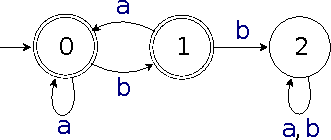
\includegraphics[width=\linewidth]{regulaer/L1.pdf}
	\end{figure}
\end{frame}

\begin{frame}
	Jetzt sieht man vielleicht auch $$G = (\{X\}, \{a, b\}, X, P )$$ mit $$P = \{X \to aX \mid baX \mid b \mid \varepsilon \}$$
\end{frame}

\begin{frame}{Noch mehr Beispiele}
	\begin{itemize}
		\item $G = (\{X \}, \{a, b\}, X , \{X \to abX \mid bbaX \mid \varepsilon \}$ wird beschrieben durch
			$L(G) = \lang{\visible<2-|handout:2>{ (ab\mid bba)\ast }} $
		\item $G = (\{X , Y\}, \{a, b\}, X , \{X \to aX \mid bX \mid ababbY , Y \to aY \mid bY \mid \varepsilon \}$ wird beschrieben durch 
			$L(G) = \lang{\visible<3-|handout:2>{ (a\mid b)\ast ababb(a\mid b)\ast }} $
	\end{itemize}
\end{frame}

\begin{frame}{Aufgabe}
	Gegeben ist im folgenden jeweils eine Beschreibung einer formalen Sprache $L$ und ein dazugehöriges Alphabet. Schreiben Sie jeweils den regulären Ausdruck $R$ auf, für den $L(R) = L $ gilt und stellen Sie eine rechtslineare Grammatik $G$ auf, für die $L(G) = L $ gilt:
	\begin{itemize}
		\item Die Menge aller Worte über dem Alphabet $A=\{a,b,c\}$, die genau ein c enthalten. \\
		\visible<2-|handout:2>{
			\emph{Lösung}: $(a|b)*c(a|b)*$
		}
		\item Die Menge aller Worte über dem Alphabet $A=\{a,b\}$, bei denen die Anzahl der $b$ durch 3 teilbar ist. \\
		\visible<3-|handout:2>{
			\emph{Lösung}: $a*(ba*ba*ba*)*$
		}
	\end{itemize}
\end{frame}

\begin{frame}{Aufgabe}
	\textit{Gegeben sei die rechtslineare Grammatik } $$ G= (\{S\},\{a,b\},S,P) \qquad P = \{S\to baaS | baS | aaS | \varepsilon \} $$
	\begin{itemize}
		\only<1-3|handout:1,2>{
			\item Geben Sie einen endlichen Akzeptor $A$ an, so dass $L(A) = L(G)$ gilt
			\only<3|handout:2>{
				\begin{figure}[H]
					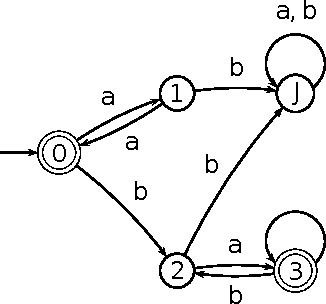
\includegraphics[scale=0.9]{regulaer/L2.pdf}
				\end{figure}
			}
		}
		\only<1,4-5|handout:1,3>{
			\item Geben Sie einen regulären Ausdruck $R$ an, so dass $ \langle R \rangle = L(G) $ gilt
			\only<5|handout:3>{
			$$ (baa|ba|aa)\ast$$
			}
		}
		\only<1,6-7|handout:1,3>{
			\item Geben Sie einen regulären Ausdruck $R$ an, der nicht das Zeichen $|$ enthält, und für den $\langle R \rangle = L(G) $ gilt.
			\only<7|handout:3>{
			$$ (aa)\ast (baa\ast)\ast $$
			}
		}
	\end{itemize}
\end{frame}



%\begin{frame}
%	\frametitle{Was wir können:}
%	Von..
%	\begin{description}
%		\item[..rechtslinearen Gammatiken..] zu
%		\begin{itemize}
%			\item den Akzeptoren: \pause (mind.) jedes Nichtterminalsymbol ein Zustand, $|$ ist Verzweigung, Akzeptierende Zustände wählen \pause
%			\item den regulären Ausdrücken: \pause Schwierig!
%		\end{itemize}
%		\item[..endlichen Akzeptoren..]  zu
%		\begin{itemize}
%			\item den Grammatiken: \pause Zustandsübergang ist eine Produktion\pause
%			\item den regulären Ausdrücken: \pause Einzelne Wege abgehen
%		\end{itemize}
%		\item[..regulären Ausdrücken..] zu
%		\begin{itemize}
%			\item den Akzeptoren: \pause in Abschnitte teilen, $\ast$ ist Schleife, $|$ ist Verzweigung \pause
%			\item den rechtslinearen Grammatiken: \pause genauso wie Akzeptor
%		\end{itemize}
%	\end{description}
%\end{frame}

% Layout: Regexe vertikal zentriert neben die Automaten geht nicht... Gnarf.
\begin{frame}{Übung: Akzeptoren und Reguläre Ausdrücke}
	Gebt graphisch einen endlichen Akzeptor sowie einen regulären Ausdruck über dem Alphabet $X=\{\word a,\word b\}$ an, der folgende Sprache akzeptiert:
	\begin{itemize}
		\item \begin{tabular}{lr}
			Die leere Menge: \visible<2-|handout:2>{\ $\lang{\rx{O}}$} \qquad \mbox{} & Die Menge des leeren Wortes: \visible<3-|handout:2>{\	$\lang{\rx{O*}}$ } \\
			\visible<2-|handout:2>{
				\scalebox{.8}{
					\begin{tikzpicture}[->,>=stealth,shorten >=1pt,auto,semithick,node distance=2cm,initial text={}]
					\tikzstyle{every state}=[]
					
					\node[initial,state] (M)                    {$m$};
					
					\path (M) edge [loop right] node {\word a, \word b} (M);
					\end{tikzpicture}
				}
			
			}
			&
			\visible<3-|handout:2>{
				\scalebox{.8}{
					\begin{tikzpicture}[->,>=stealth,shorten >=1pt,auto,node distance=2cm,
					semithick,initial text={}]
					\tikzstyle{every state}=[]
					
					\node[initial,state,accepting] (A)                    {$a$};
					\node[state]		 		   (M)  [right of=A]		{$m$};
					
					\path
					(A) edge 			  node {\word a, \word b} (M) 
					(M) edge [loop right] node {\word a, \word b} (M);
					\end{tikzpicture}
			}
		}
		\end{tabular}  
		\item Die Menge aller Worte, die genau ein \word b enthalten:
		\visible<4-|handout:2>{\ $\lang{\rx{a*ba*}}$ \\
			\scalebox{.8}{
				\begin{tikzpicture}[->,>=stealth,shorten >=1pt,auto,node distance=2cm,
				semithick,initial text={}]
				\tikzstyle{every state}=[]
				
				\node[initial,state] (A)                    {$a$};
				\node[state,accepting] (B)  [right of=A]     {$b$};
				\node[state]		 (M)  [right of=B]		{$m$};
				
				\path
				(A) edge [loop above]  node {\word a} (A) 
				(A) edge 			  node {\word b} (B) 
				(B) edge [loop above]  node {\word a} (B) 
				(B) edge 			  node {\word b} (M) 
				(M) edge [loop above] node {\word a, \word b} (M);
				\end{tikzpicture}
		}
	
	}
		\item Die Menge aller Worte, bei denen die Anzahl der $\word b$ durch 3 teilbar ist: 
		\visible<5-|handout:2>{ 
			\begin{minipage}[t]{.5\linewidth}
				\vspace{-\ht\strutbox} \scalebox{.8}{\begin{tikzpicture}[->,>=stealth,shorten >=1pt,auto,node distance=2cm,
				semithick,initial text={}]
				\tikzstyle{every state}=[]
				
				\node[initial,state,accepting] (0)                    {$0$};
				\node[state] (1)  [right of=A]     {$1$};
				\node[state]		 (2)  [right of=B]		{$2$};
				
				\path
				(0) edge [loop above]  node {\word a} (0) 
				(0) edge 			  node {\word b} (1) 
				(1) edge [loop above]  node {\word a} (1) 
				(1) edge 			  node {\word b} (2) 
				(2) edge [loop right] node {\word a} (2)
				(2) edge [bend left]  node {\word b} (0) ;
				\end{tikzpicture}}	
				
			\end{minipage} 
			 $\lang{\rx{(a*ba*ba*b)*a*}}$ 
	}
	\end{itemize}
\end{frame}

% Dieses Jahr nicht
%input{../Bloecke/StrukturelleInduktion}

\begin{frame}	
	\begin{block}{Was ihr nun wissen solltet}
		\begin{itemize}
			\item Wie man rekursive Laufzeiten mastert
			\item Endlich: Automaten!
			\item ...und wie man damit Wörter akzeptiert/ablehnt
			\item Nicht immer so vulgär: Reguläre Ausdrücke
		\end{itemize}
	\end{block}
	
	\begin{block}{Was nächstes Mal kommt}
		\begin{itemize}
			\item Rechtslineare Grammatiken
			\item Turingmaschinen
			%\item Turingmaschinen -- mächtiger wird es nicht mehr!
		\end{itemize}
	\end{block}
\end{frame}

\lastframe{0.6}{30}{xkcd/automation_1319.png}{http://www.xkcd.com/1319}
%\xkcdframe{0.5}{30}{xkcd/houston_1438.png}{http://www.xkcd.com/1438}{Oh, hi mom. No, nothing important, just work.}

\slideThanks

\end{document}